\chapter{面向模型推理的云边协同调度系统}

本章将对面向模型推理的云边协同调度系统进行介绍。首先介绍了系统的运行平台KubeEdge的相关细节,接着介绍系统架构设计以及各个组件的设计。

\section{KubeEdge及相关技术介绍}

本文提出的面向模型推理的云边协同调度具有普适性,能够适配各类云边云原生平台。为验证其有效性,需选择具有典型代表性的云边协同平台进行落地和验证。KubeEdge作为首个获得CNCF基金会认证的边缘计算框架,其架构设计深度契合云边协同的分布式计算范式,且由华为主导的活跃开源社区持续提供技术演进保障。因此,本文选择基于KubeEdge构建KEAS系统。

\subsection{KubeEdge架构设计}

KubeEdge是一种面向云边协同场景的边缘计算框架,旨在将Kubernetes的能力从云端延伸至边缘,从而实现统一的资源管理和应用部署。如图 \ref{fig:4-1kubeedge} 所示,KubeEdge通过云端和边缘组件的紧密协作,构建了一个高效且可靠的分布式架构。该架构不仅支持边缘节点的自治运行,还能在网络条件受限的情况下保持与云端的稳定通信。

\begin{figure}[ht]
  \centering
  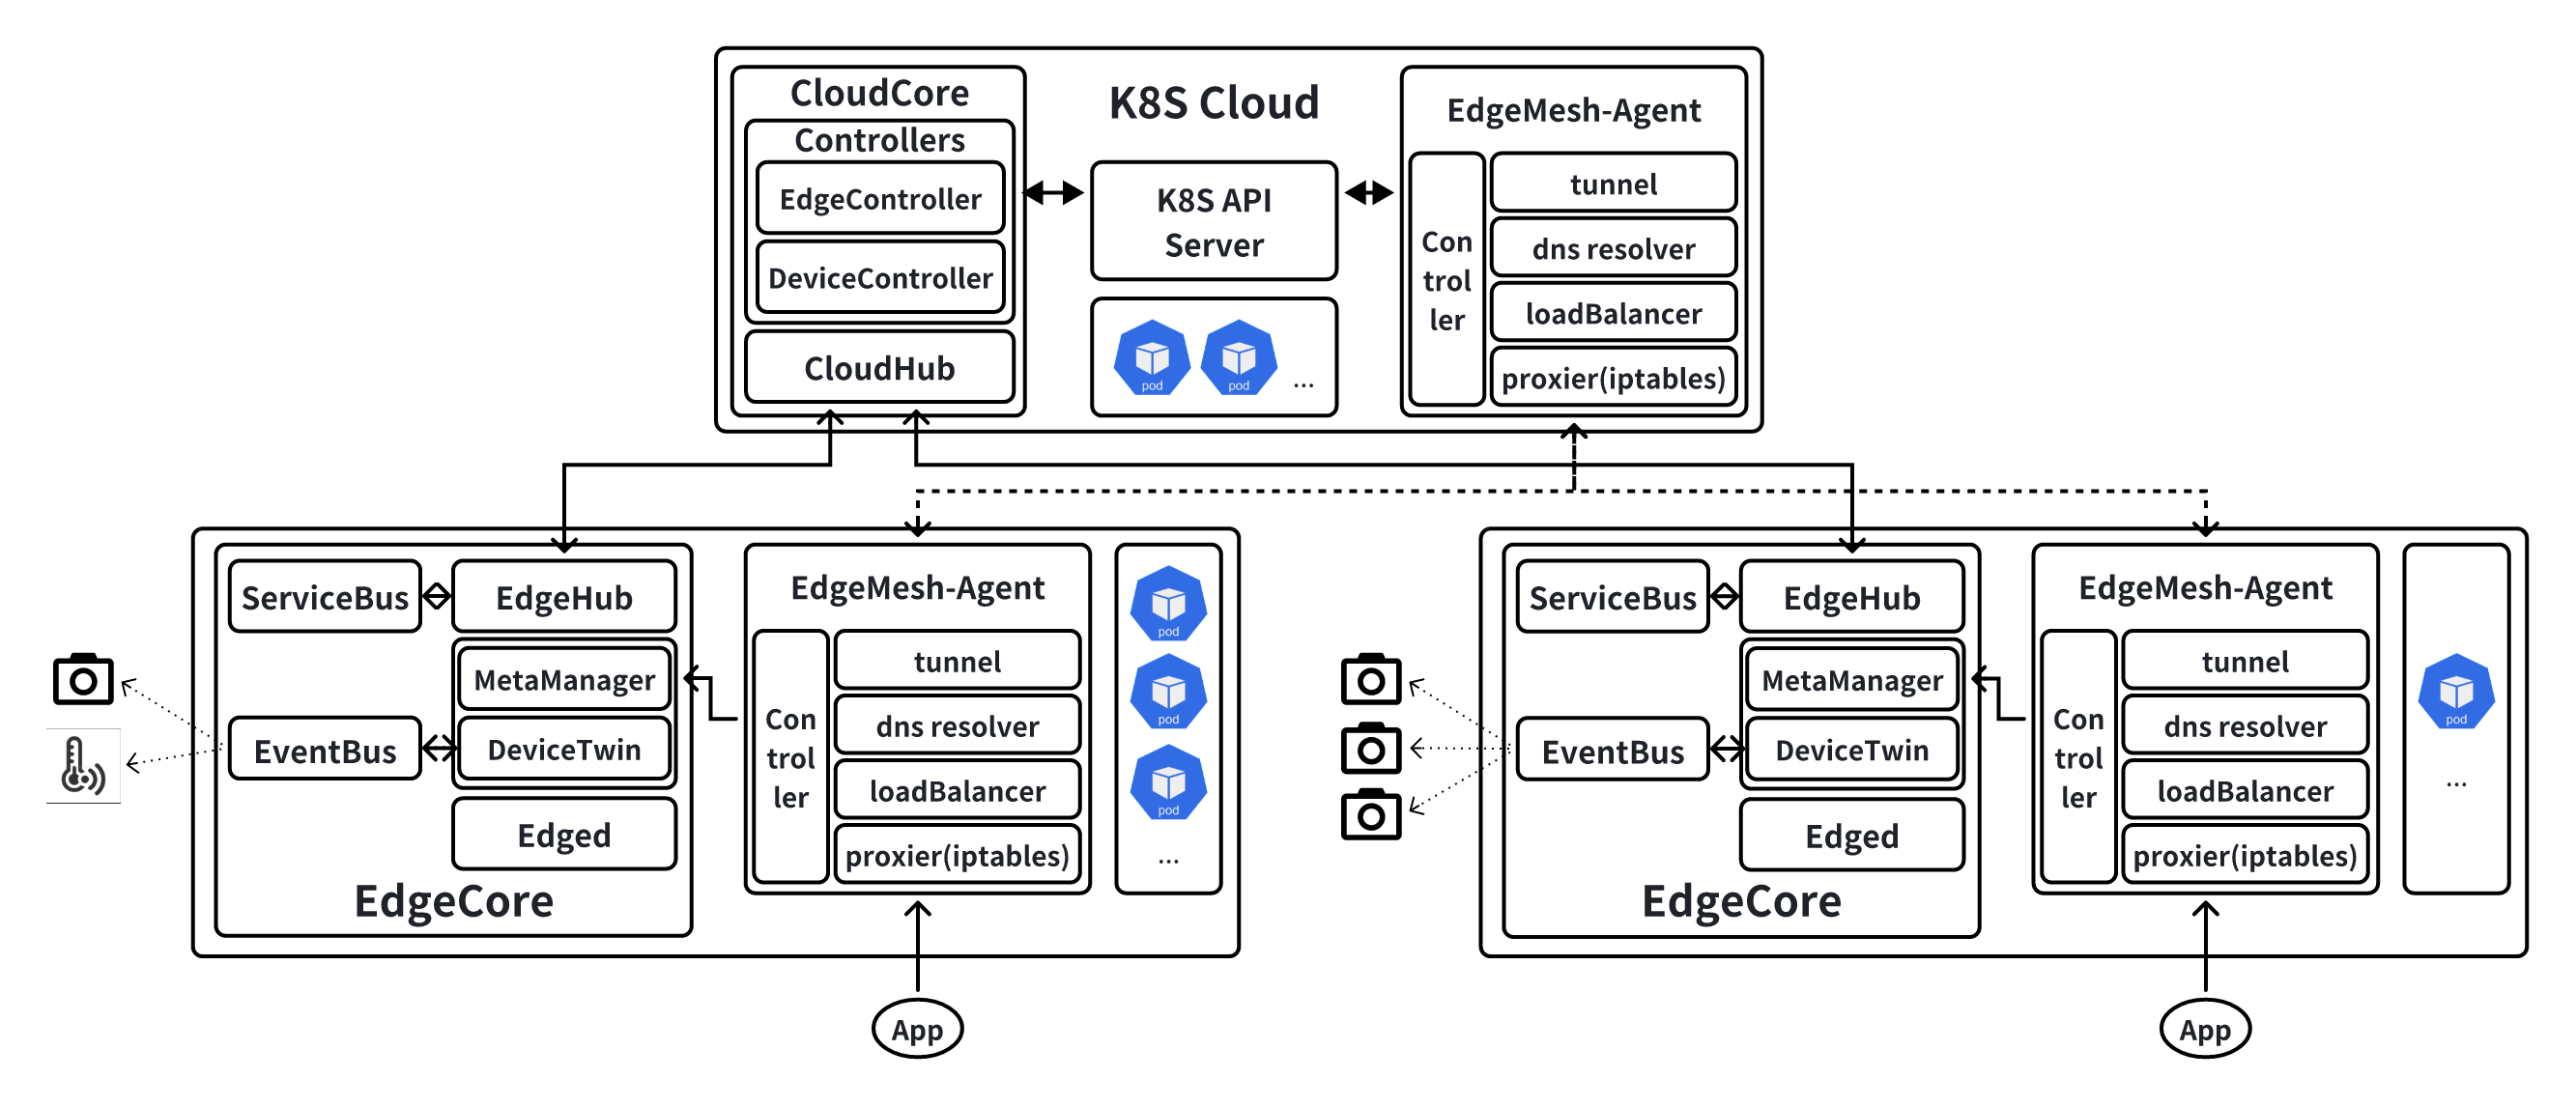
\includegraphics[width=\textwidth]{pics/4-1kubeedge.png}
  \caption{KubeEdge系统架构\cite{xiong2018extend}}
  \label{fig:4-1kubeedge}
\end{figure}

% \begin{figure}[ht]
%   \centering
%   \begin{adjustbox}{center, max width=1.2\textwidth}
%     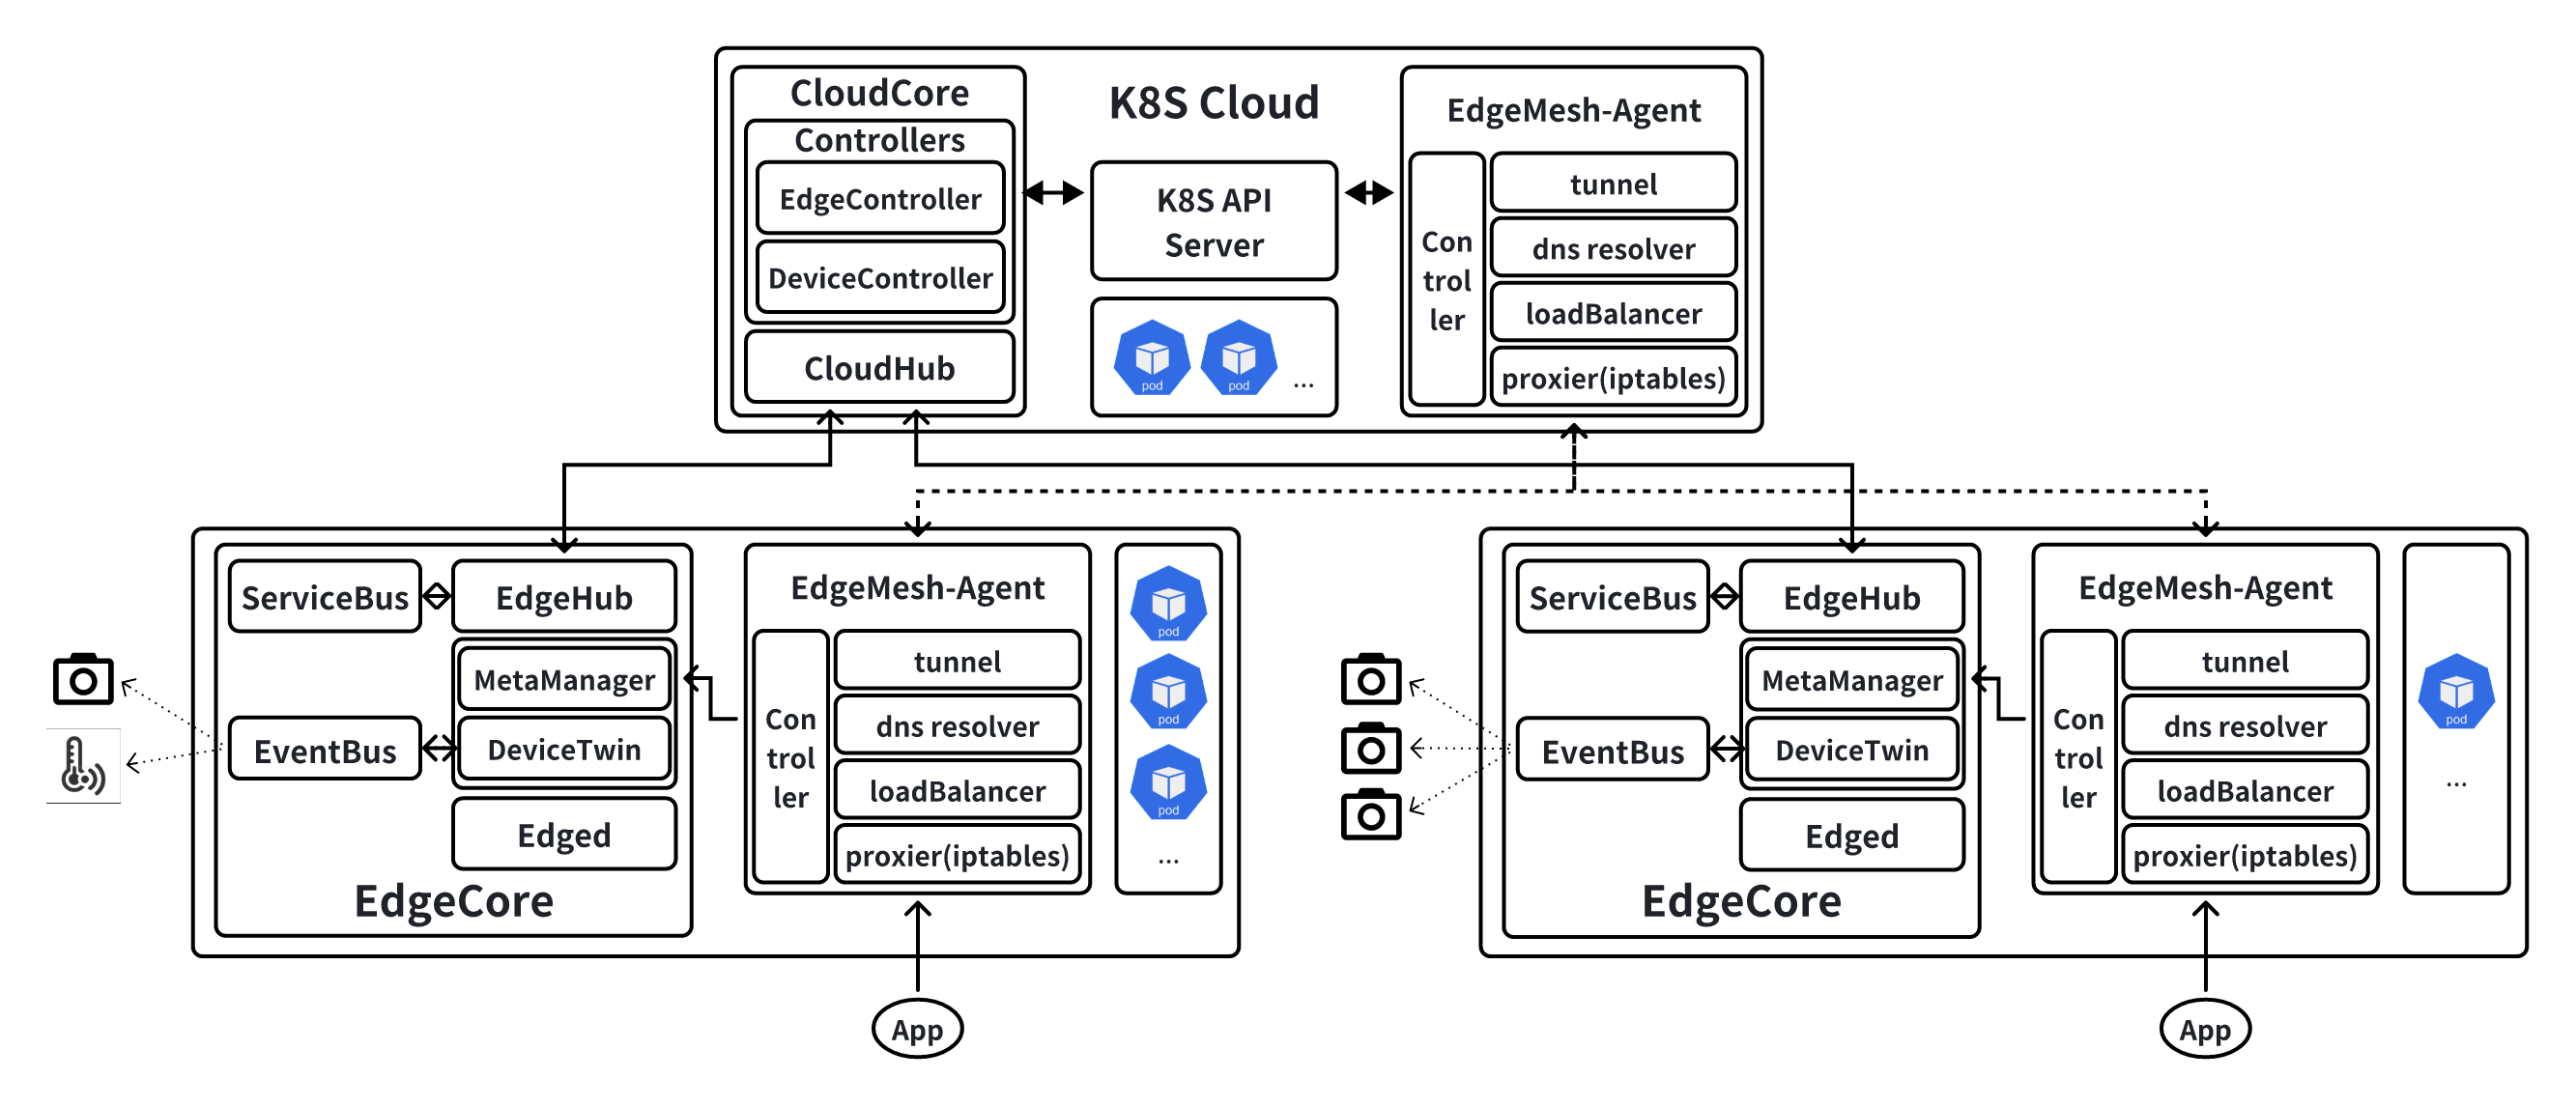
\includegraphics{pics/4-1kubeedge.png}
%   \end{adjustbox}
%   \caption{KubeEdge系统架构\cite{xiong2018extend}}
%   \label{fig:4-1kubeedge}
% \end{figure}


KubeEdge的核心功能依赖于云端和边缘组件的协同工作。云端的边缘控制器(Edge Controller)与边缘侧的EdgeHub组件共同实现了基于事件驱动的双向同步机制。这一机制通过 Kubernetes API Server 与 EdgeCore 的交互,确保了云边节点的状态一致性,同时支持边缘节点注册、服务部署及资源状态的实时更新。此外,CloudHub 和 EdgeHub 组件通过双向 WebSocket 连接构建了分布式消息总机,采用消息缓存与断点续传技术,有效应对网络波动带来的挑战,从而保证通信的可靠性。

在边缘端,KubeEdge通过EdgeD和MetaManager共同支撑轻量化的计算基础设施。EdgeD作为核心执行引擎,深度集成容器运行时接口(CRI),实现了对Pod工作负载的全生命周期管理,涵盖资源调度、机密注入及健康监测等关键功能。MetaManager则作为EdgeD的辅助模块,负责元数据的存储与检索。两者通过分层缓存策略优化了存储效率与访问性能:高频访问的元数据存储在内存数据库中,低频数据则持久化至SQLite。这种设计使得KubeEdge能够在资源受限的边缘环境中高效运行,同时保持与云原生生态的无缝对接。

KubeEdge的设备管理和服务通信能力是其另外两项重要特性,将在后续章节中详细阐述。

\subsection{设备管理模块}

KubeEdge的设备管理模块通过数字孪生技术实现物理设备与虚拟对象的双向映射。如图\ref{fig:4-2mapper}所示,设备控制器(Device Controller)基于Kubernetes CRD机制定义设备抽象模型(Device CRDs),通过声明式API实现设备状态的云端声明与边缘同步。该模块与边缘组件DeviceTwin形成闭环:Mapper框架负责设备数据的采集与协议转换,DeviceTwin将采集数据映射为数字孪生体的状态属性并存储于本地数据库,EdgeHub则通过WebSocket通道将设备状态更新同步至云端。

\begin{figure}[ht]
  \centering
  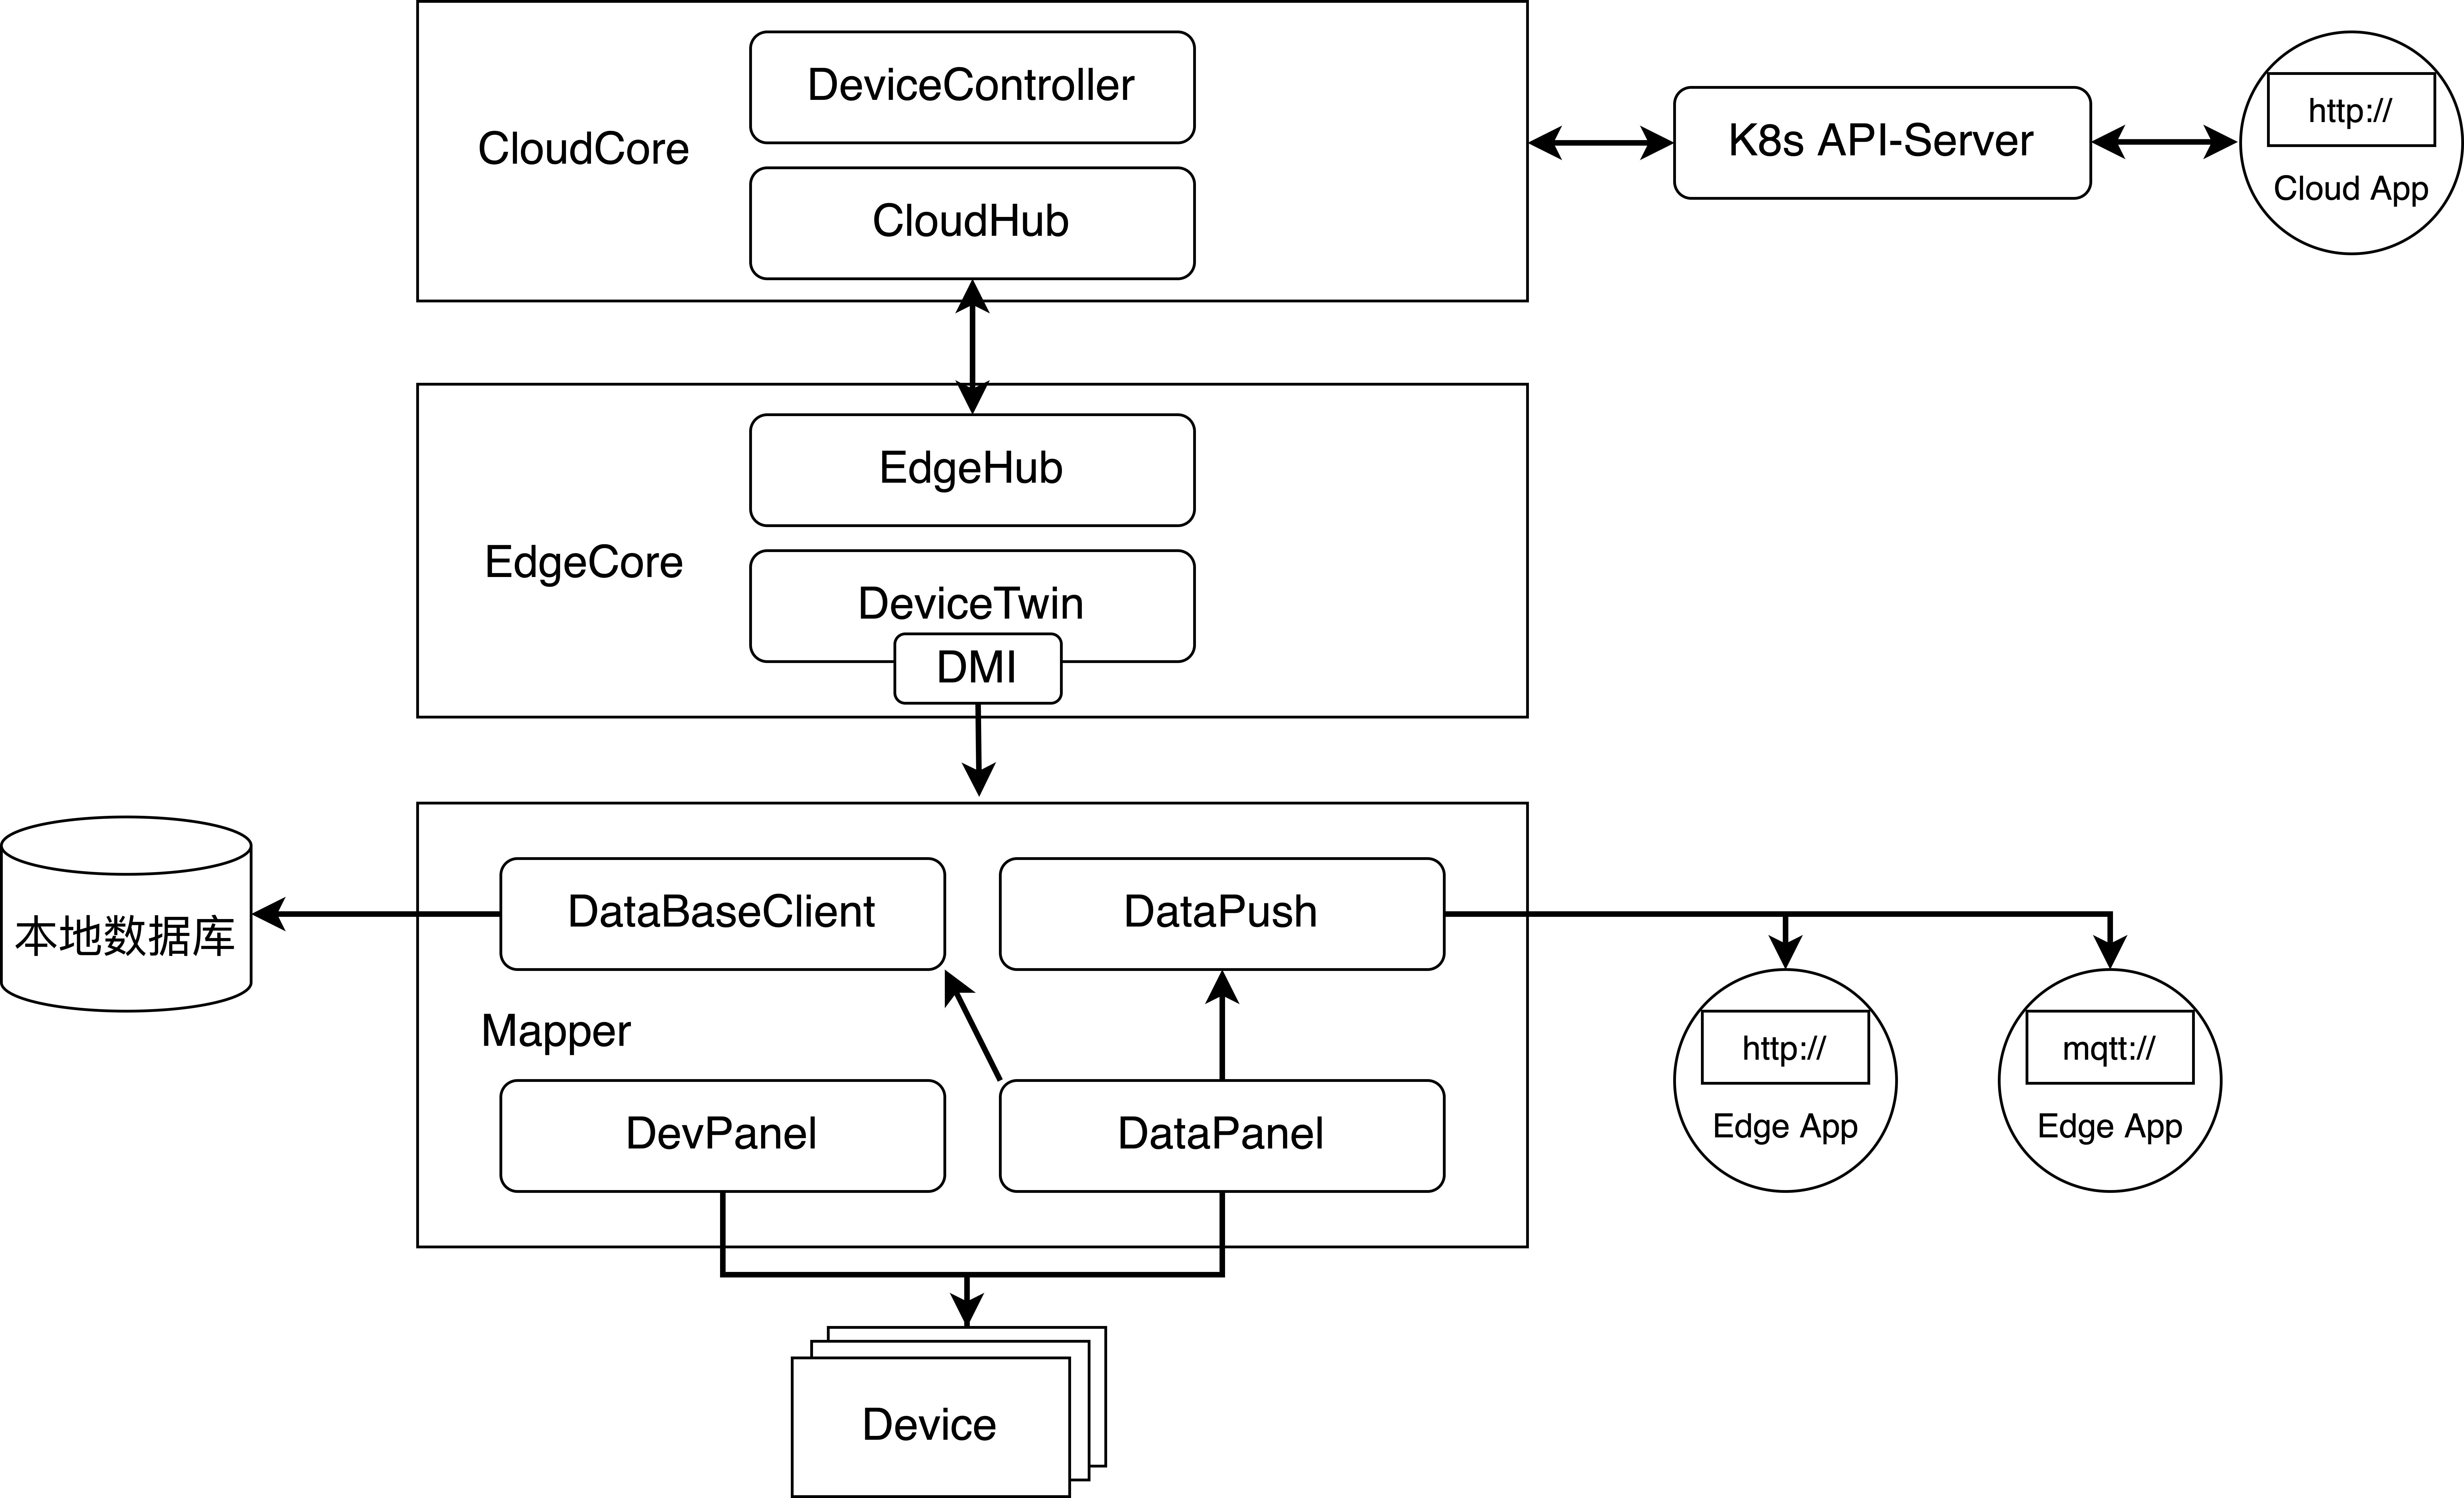
\includegraphics[width=\linewidth]{pics/4-2mapper.png}
  \caption{KubeEdge设备管理架构\cite{xiong2018extend}}
  \label{fig:4-2mapper}
\end{figure}

在 KubeEdge 的设计中,Mapper 框架不仅支持设备平面(DevPanel)的设备运行管理,提供设备数据的采集与协议转换功能,还在数据平面(DataPanel)上提供了灵活的数据推送能力。采集到的设备数据可以通过 MQTT 协议实时推送到消息队列中,以满足实时数据分析的需求;同时,Mapper 还支持将数据推送到时序数据库(如 InfluxDB)中,以便进行高效的时序数据分析与长期存储。这种设计使得KubeEdge能够高效地应对高频率、多源异构的设备数据流,并根据任务需求动态调整数据处理路径,从而实现云边协同中的资源优化与性能提升。

本文利用 KubeEdge 提供的 Device CRDs 和 Mapper 框架模块来管理终端设备。具体而言,Device CRDs 用于描述设备的静态属性和能力,这些属性包括设备的功能特性、通信协议以及数据格式等信息。Mapper 框架则负责实现设备的动态数据采集逻辑,支持根据预定义的采集策略或外部事件触发机制动态调整数据采集行为。

\subsection{基于EdgeMesh的服务通信}

EdgeMesh 是 KubeEdge 集群中用于实现服务发现和跨节点通信的核心组件,其设计目标是解决边缘计算场景下节点间通信的复杂性和不稳定性问题。在边缘计算环境中,网络条件通常受限,尤其是弱网环境下的跨局域网通信需求更为突出。为应对这一挑战,EdgeMesh 基于 LibP2P 技术构建了一套去中心化的通信网络。该网络能够动态适应网络拓扑的变化,从而在边缘节点之间建立高效、可靠的数据传输通道。

在局域网内,EdgeMesh 支持直接访问的方式完成节点间的数据交互;而在跨局域网场景下,EdgeMesh 通过 NAT 打洞技术或中继流量的方式实现节点间的通信。此外,EdgeMesh 借助 EdgeHub - CloudHub 隧道分发元数据,避免了对云端的直接访问,从而显著降低了云端的负载压力。为了进一步提升服务发现的可靠性,EdgeMesh 在每个节点上部署了轻量级的 DNS 服务器。这种设计确保了服务搜索的高效性和准确性,同时支持动态更新和分布式管理。

本文利用 EdgeMesh 的服务发现功能和跨节点通信能力,实现了节点之间调度模块的高效通信。具体而言,EdgeMesh 的去中心化通信网络为跨节点的调度决策提供了低延迟、高可靠的数据传输通道。此外,EdgeMesh 的服务发现机制通过轻量级 DNS 服务器的支持,为流式数据的转发提供了支撑,使其在边缘节点间的高效传递。

\begin{figure}[ht]
  \centering
  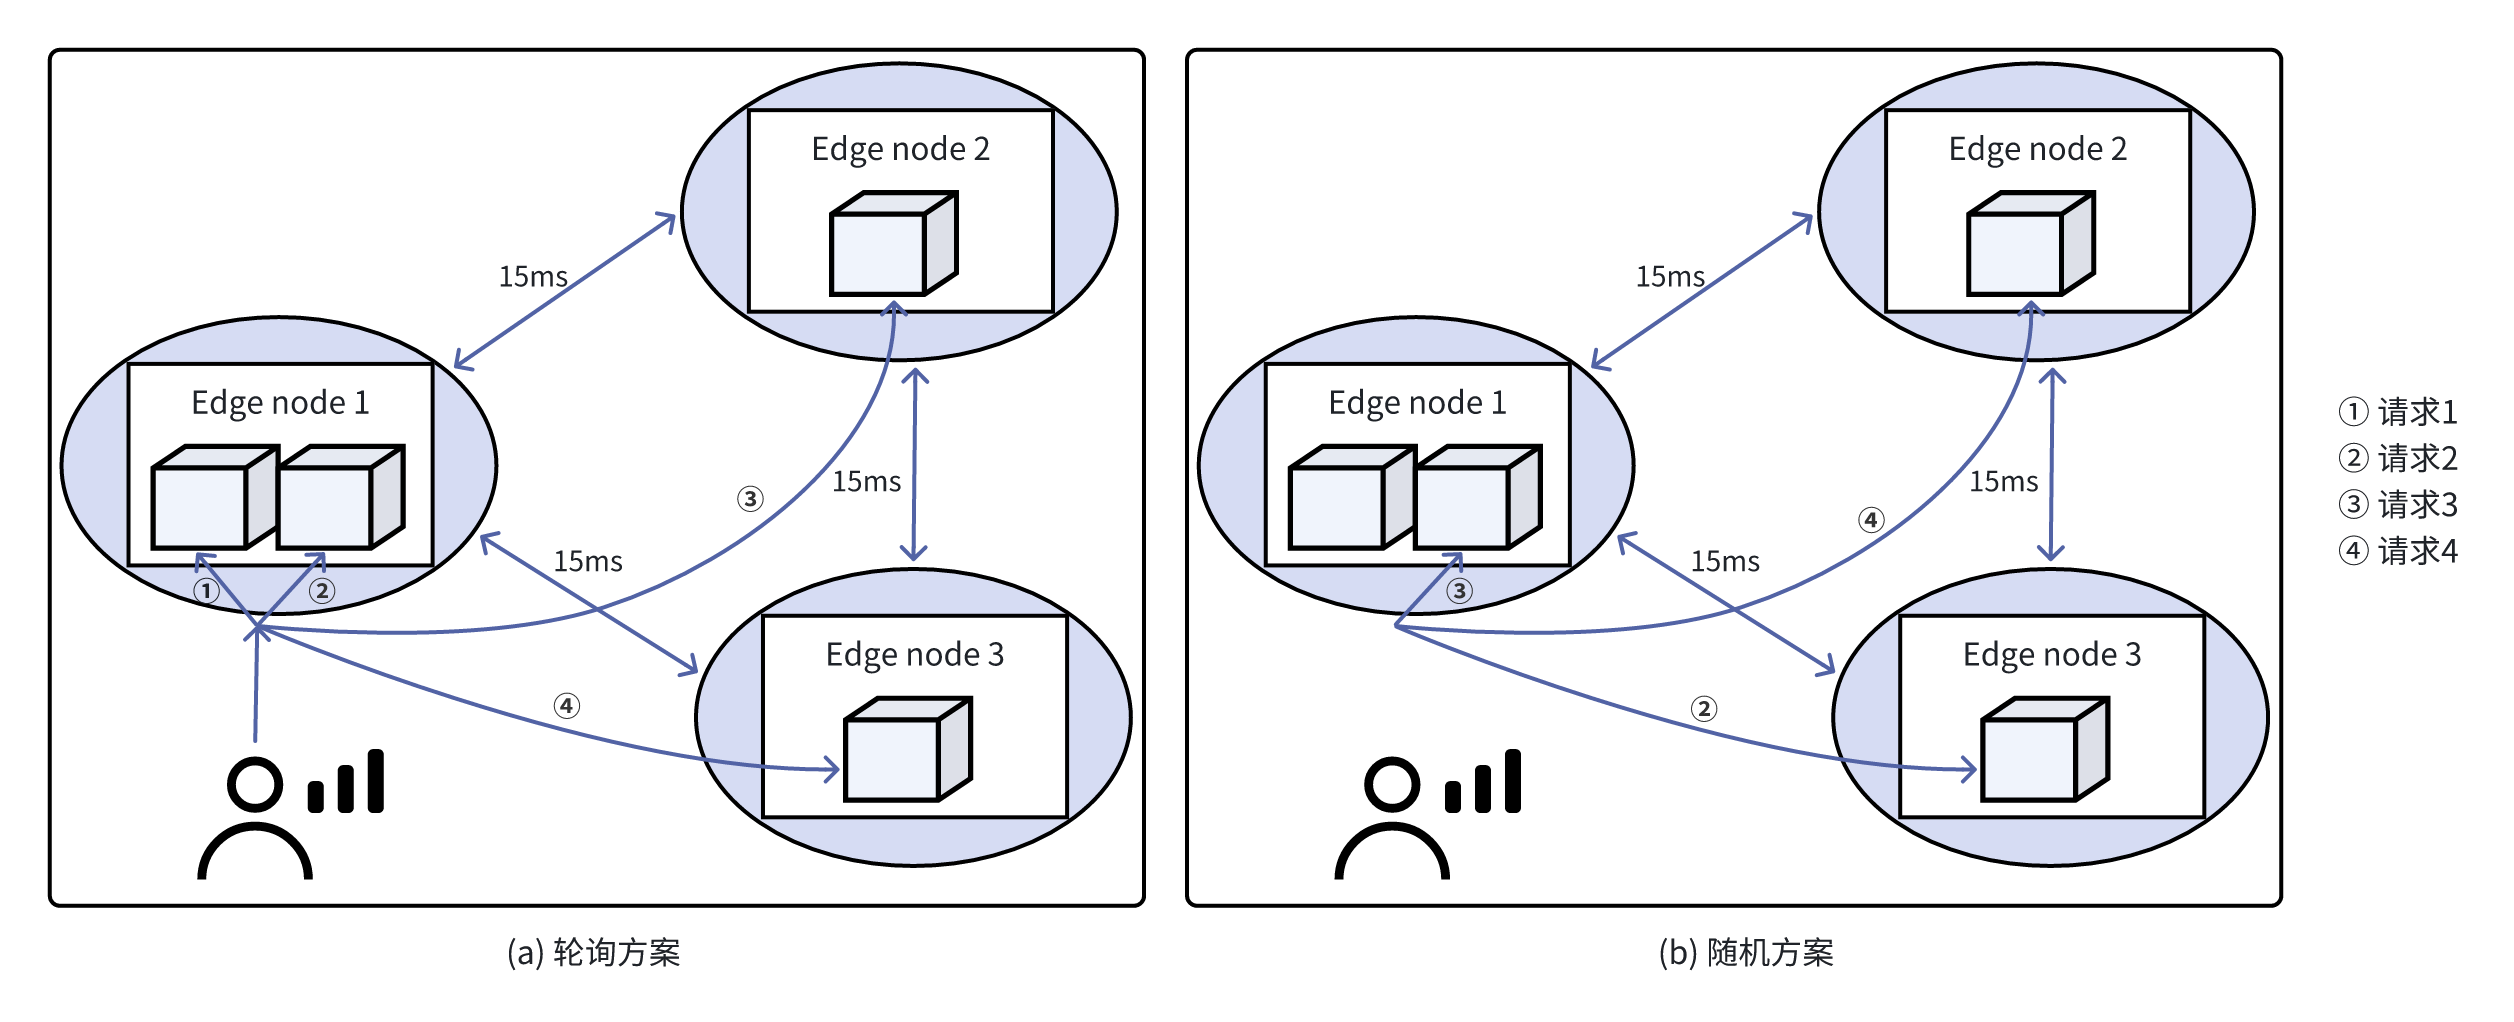
\includegraphics[width=\linewidth]{pics/4-3edgemesh.png}
  \caption{KubeEdge 中的负载均衡方案}
  \label{fig:4-3edgemesh}
\end{figure}

在负载均衡方面,EdgeMesh 目前采用 Istio 的目标规则(DestinationRule),并支持轮询和随机分配等基础策略,以实现流量在各 Pod 间的高效分发,如图 \ref{fig:4-3edgemesh} 所示。然而,在云边协同 AI 推理场景中,边缘节点分布广、网络异构性高,这种传统的负载均衡方式因未考虑节点实时负载、网络质量差异及资源异构性,可能导致任务分配不均或资源利用率低下。

\section{系统架构设计}

在第三章的基础上,本文提出了一种基于 KubeEdge 的原型系统 KEAS。该系统的核心在于实现了分层的调度机制。为支持这一复杂的调度机制,KEAS 在 KubeEdge 平台上构建了一个 Akka 集群,并在物理的三层拓扑上构建了分层的逻辑拓扑,以实现高效的调度管理。同时,利用 Akka Actor 模型实现设备数据流请求的高效转发与模块间通信。Actor 模型通过异步消息传递机制避免了传统多线程编程中的锁竞争问题,从而显著提升了系统的并发性能和可靠性。此外,其异步通信特性能够有效应对云边协同场景中网络延迟和不稳定的问题,确保消息传递的可靠性和低延迟。为实现 Akka 集群与 KubeEdge 的深度集成,本文设计了监听协调模块。该模块通过 Kubernetes 的 Informer 机制实时监控集群状态,并调用 Kubernetes API 动态部署和管理关键负载。

\begin{figure}[ht]
  \centering
  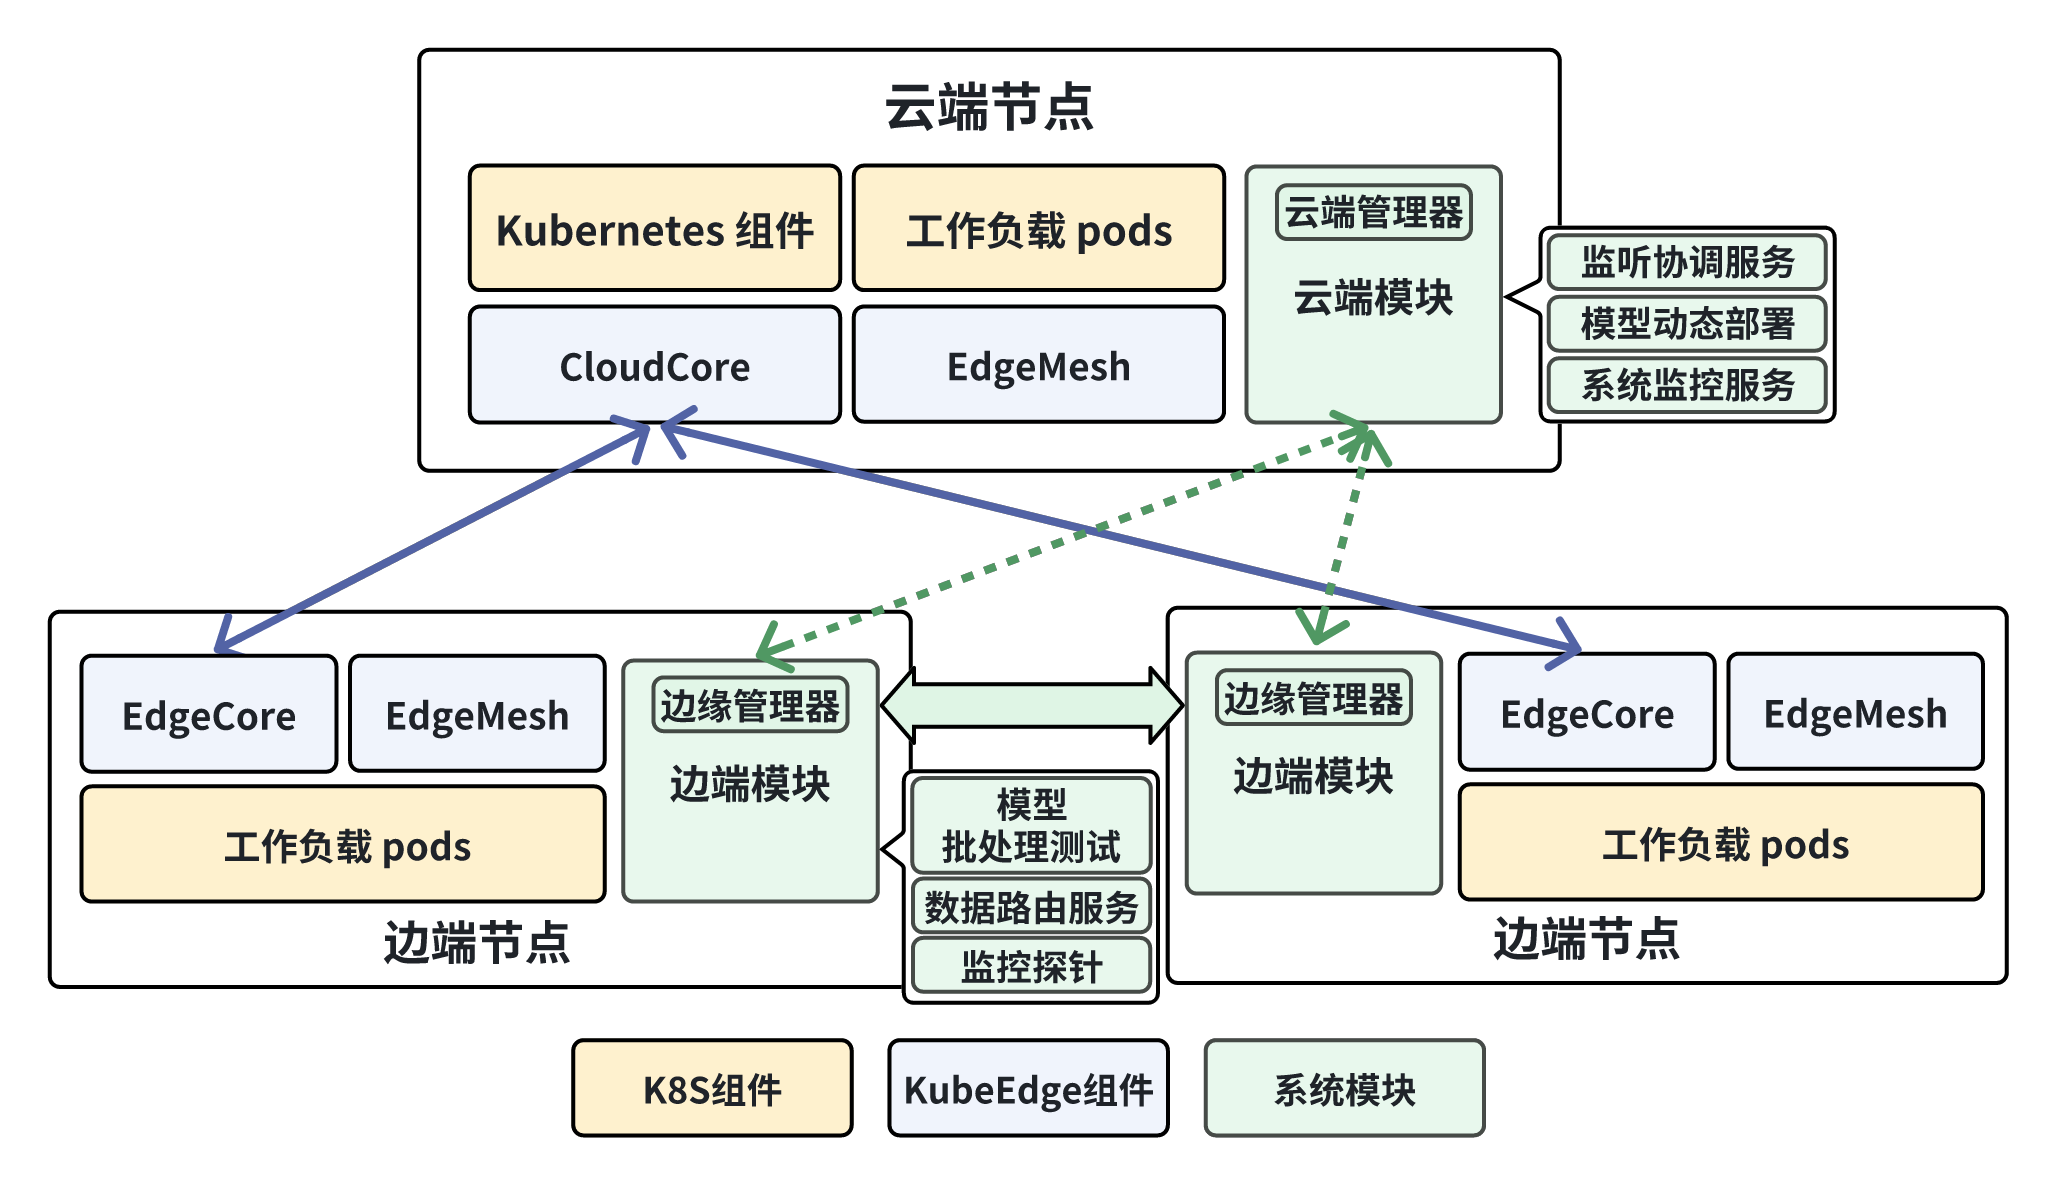
\includegraphics[width=\linewidth]{pics/4-4系统架构.png}
  \caption{KEAS 系统架构}
  \label{fig:4-4arch}
\end{figure}

系统的整体架构如图 \ref{fig:4-4arch} 所示。KEAS 系统首先需要在异构化节点上部署 AI 模型,并针对不同节点的计算能力优化模型运行参数。为此,本文引入了一个AI模型批处理测试模块,在 AI 模型部署阶段对节点进行性能评估。该模块通过测试不同批处理大小下的AI模型推理性能,记录每个节点在处理特定负载时的最优批处理大小及对应的运行时间。这些数据为后续调度策略的制定提供了重要依据。同时,系统通过监控探针实时采集集群节点之间的网络状况和节点运行状态。在云端,系统监控模块汇总并展示每个节点的运行状态以及节点间的网络通信情况,为调度决策提供全面的数据支持。基于上述数据采集与分析,KEAS 系统实现了分层调度策略的关键数据输入。针对调度结果,边端模块进一步实现了数据流转发路由功能,将设备流式数据高效地转发至相关节点进行处理。

具体而言,系统中的关键组件包括:

\begin{itemize}
    \item \textbf{基于 Akka 的调度服务:} 该服务基于Akka Cluster构建的核心调度模块,由云端管理器(Master)和边缘管理器(Manager)组成,支持云端全局调度和边缘节点的分层调度。云端管理器负责执行全局调度策略和动态部署模型推理实例,同时维护节点运行状态与全局网络信息,为系统提供统一的调度视图和全局资源管理能力。边缘管理器则部署在边缘节点上,主要职责是高效调度本地任务;此外,边缘管理器还能根据用户需求动态组建分层结构,实现边缘节点间的协同管理和资源优化利用。
    \item \textbf{监听协调服务:} 该服务的核心功能是实现 Kubernetes 集群中的资源感知与动态部署。该服务利用 Kubernetes 的 Informer 机制,实时捕获设备状态和集群原生资源的变更信息,并根据这些信息触发相应的记录或调度操作。例如,在节点加入集群时,系统会记录其架构信息;当设备状态发生更新时,可能触发调度流程以适应新的资源环境。此外,核心资源部署机制通过预置的标准化部署模板,自动化完成负载实例的创建、配置与管理,从而显著简化了云边协同环境中复杂的资源调度与部署任务。
    \item \textbf{模型推理服务:} 该服务聚焦于推理部署环节,有效解决了模型跨框架兼容性、硬件异构性以及动态部署等关键问题。具体而言,通过预先为不同硬件架构打包适配的推理服务镜像,并结合 Kubernetes 的节点标签机制,确保镜像与目标节点的兼容性。同时,设计了模型转换模块,支持不同框架之间的模型相互转换。在完成模型实例的动态部署后,系统通过批处理测试对推理性能进行优化,并记录批处理大小和单次运行时间等相关数据,为后续调度服务提供可靠的数据支持。
    \item \textbf{数据路由服务:} 该服务是实现高效数据分发与处理的核心组件,通过订阅 MQTT 消息代理获取设备数据,并依据调度服务生成的路由规则确定数据流向。数据会被传递至本地模型推理实例以完成后续处理,或者在需要时转发至其他节点的 MQTT 消息代理,从而实现跨节点的数据流转。
    \item \textbf{系统监控服务:} 该服务提供全面的监控功能,包括网络监控和队列监控,实时采集节点间的网络状况和节点运行状态,为调度决策提供数据支持。监控服务通过可视化界面展示集群的运行状态,帮助相关人员快速定位问题并优化资源配置。
\end{itemize}

\section{系统组件设计}

\subsection{基于 Akka 的调度服务}

在本系统中,终端设备的数据采集任务已由 KubeEdge 平台完成。为了实现分布式节点之间的状态同步以及高效的任务分发,本文在 KubeEdge 平台上构建了一个基于 Akka Cluster 的分布式调度服务。该调度服务不仅作为系统的核心调度组件,还承担了运行时状态管理与消息传递等关键职责,是整个系统的基础架构。

\begin{figure}[ht]
  \centering
  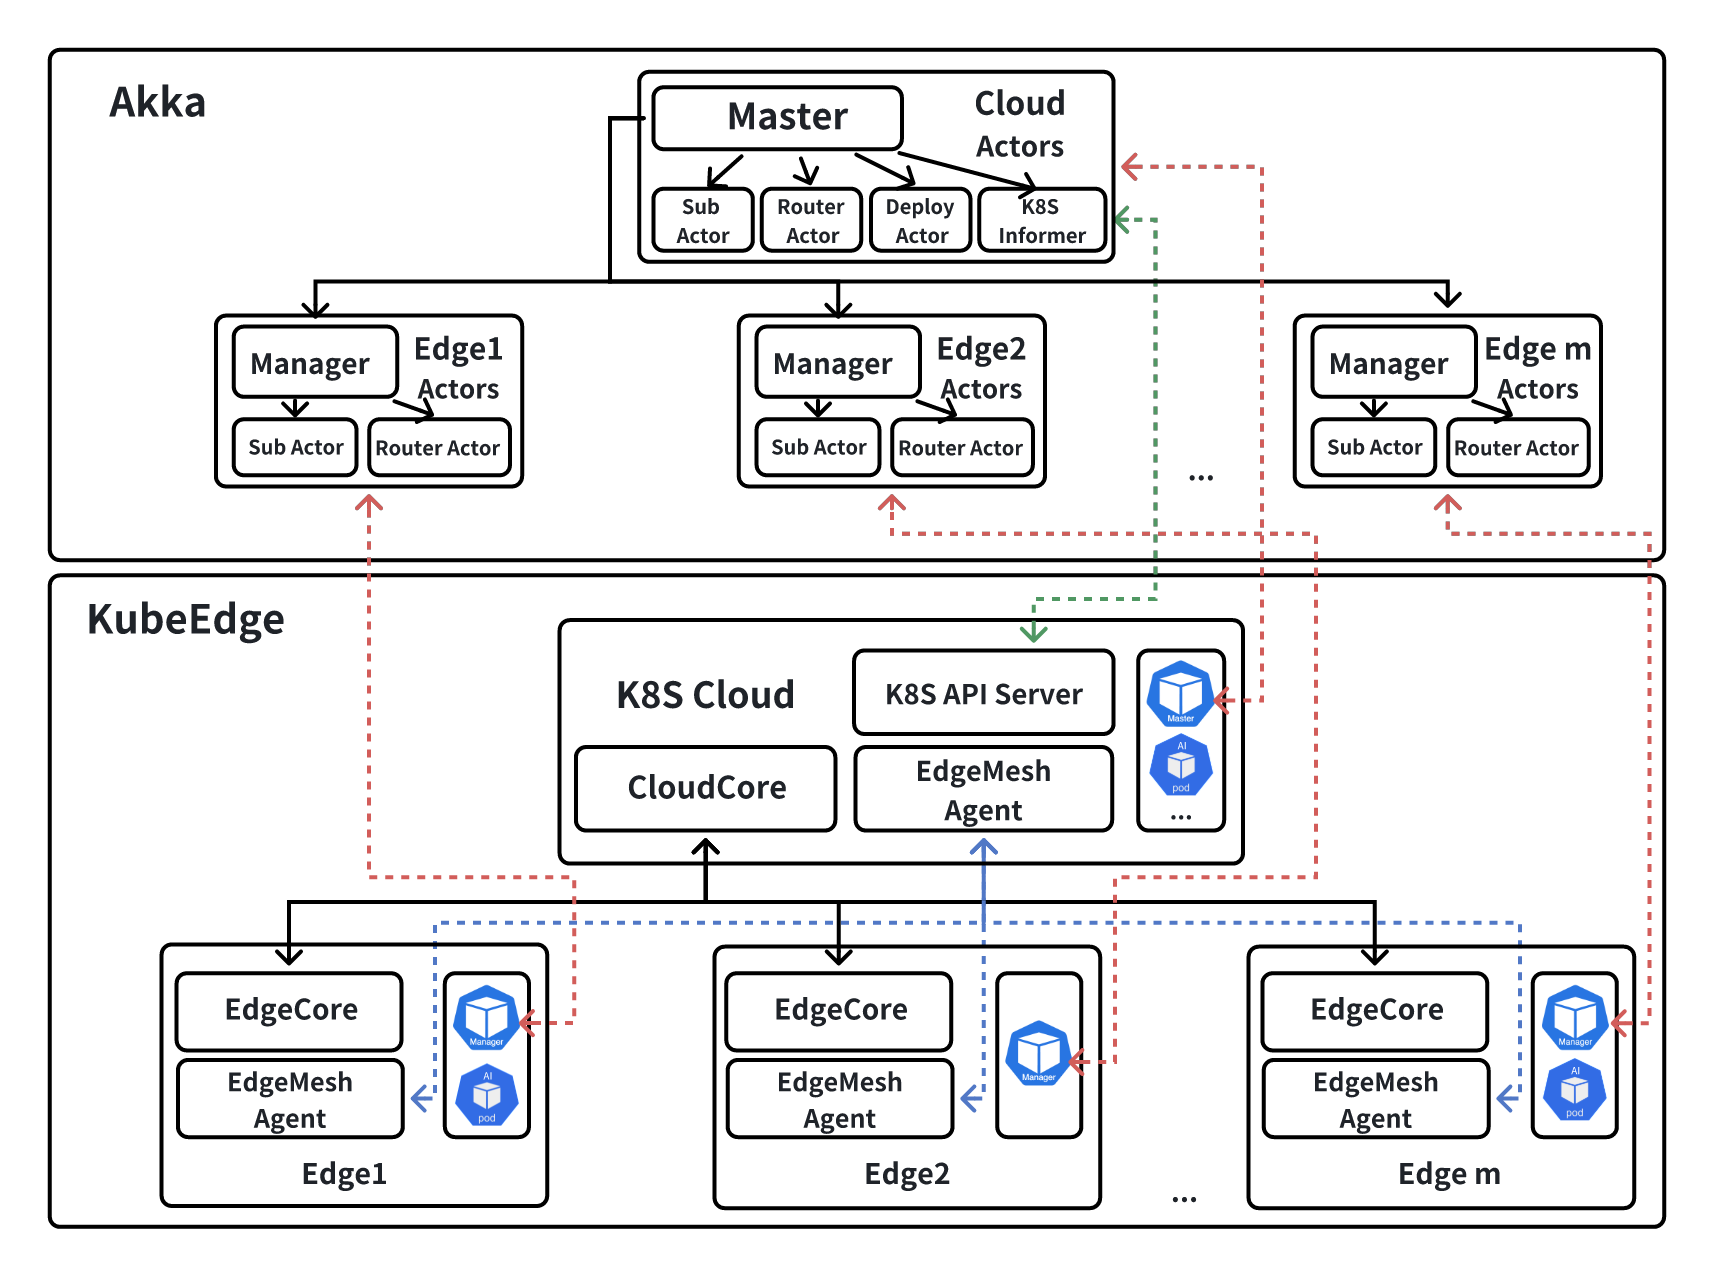
\includegraphics[width=\linewidth]{pics/4-5akka.png}
  \caption{基于 Akka 的调度服务架构}
  \label{fig:4-5akka}
\end{figure}

如图 \ref{fig:4-5akka} 所示,Akka 集群架构主要由云端管理器(Master)和边缘管理器(Manager)组成,两者通过 Akka Cluster 连接。云端管理器部署于云端节点,承担全局调度策略的执行职责。它不仅需要维护各节点上模型推理实例的运行状态,还需掌握全局网络信息。具体而言,运行状态涵盖批处理大小、单次运行时长及队列长度等关键指标。这些数据为第三章所述调度算法在云端层次的应用提供了基础支持。此外,云端管理器还负责动态部署模型推理实例,该过程将在后续章节关于监听协调服务与模型推理实例动态部署的部分中进一步探讨。

\begin{figure}[ht]
  \centering
  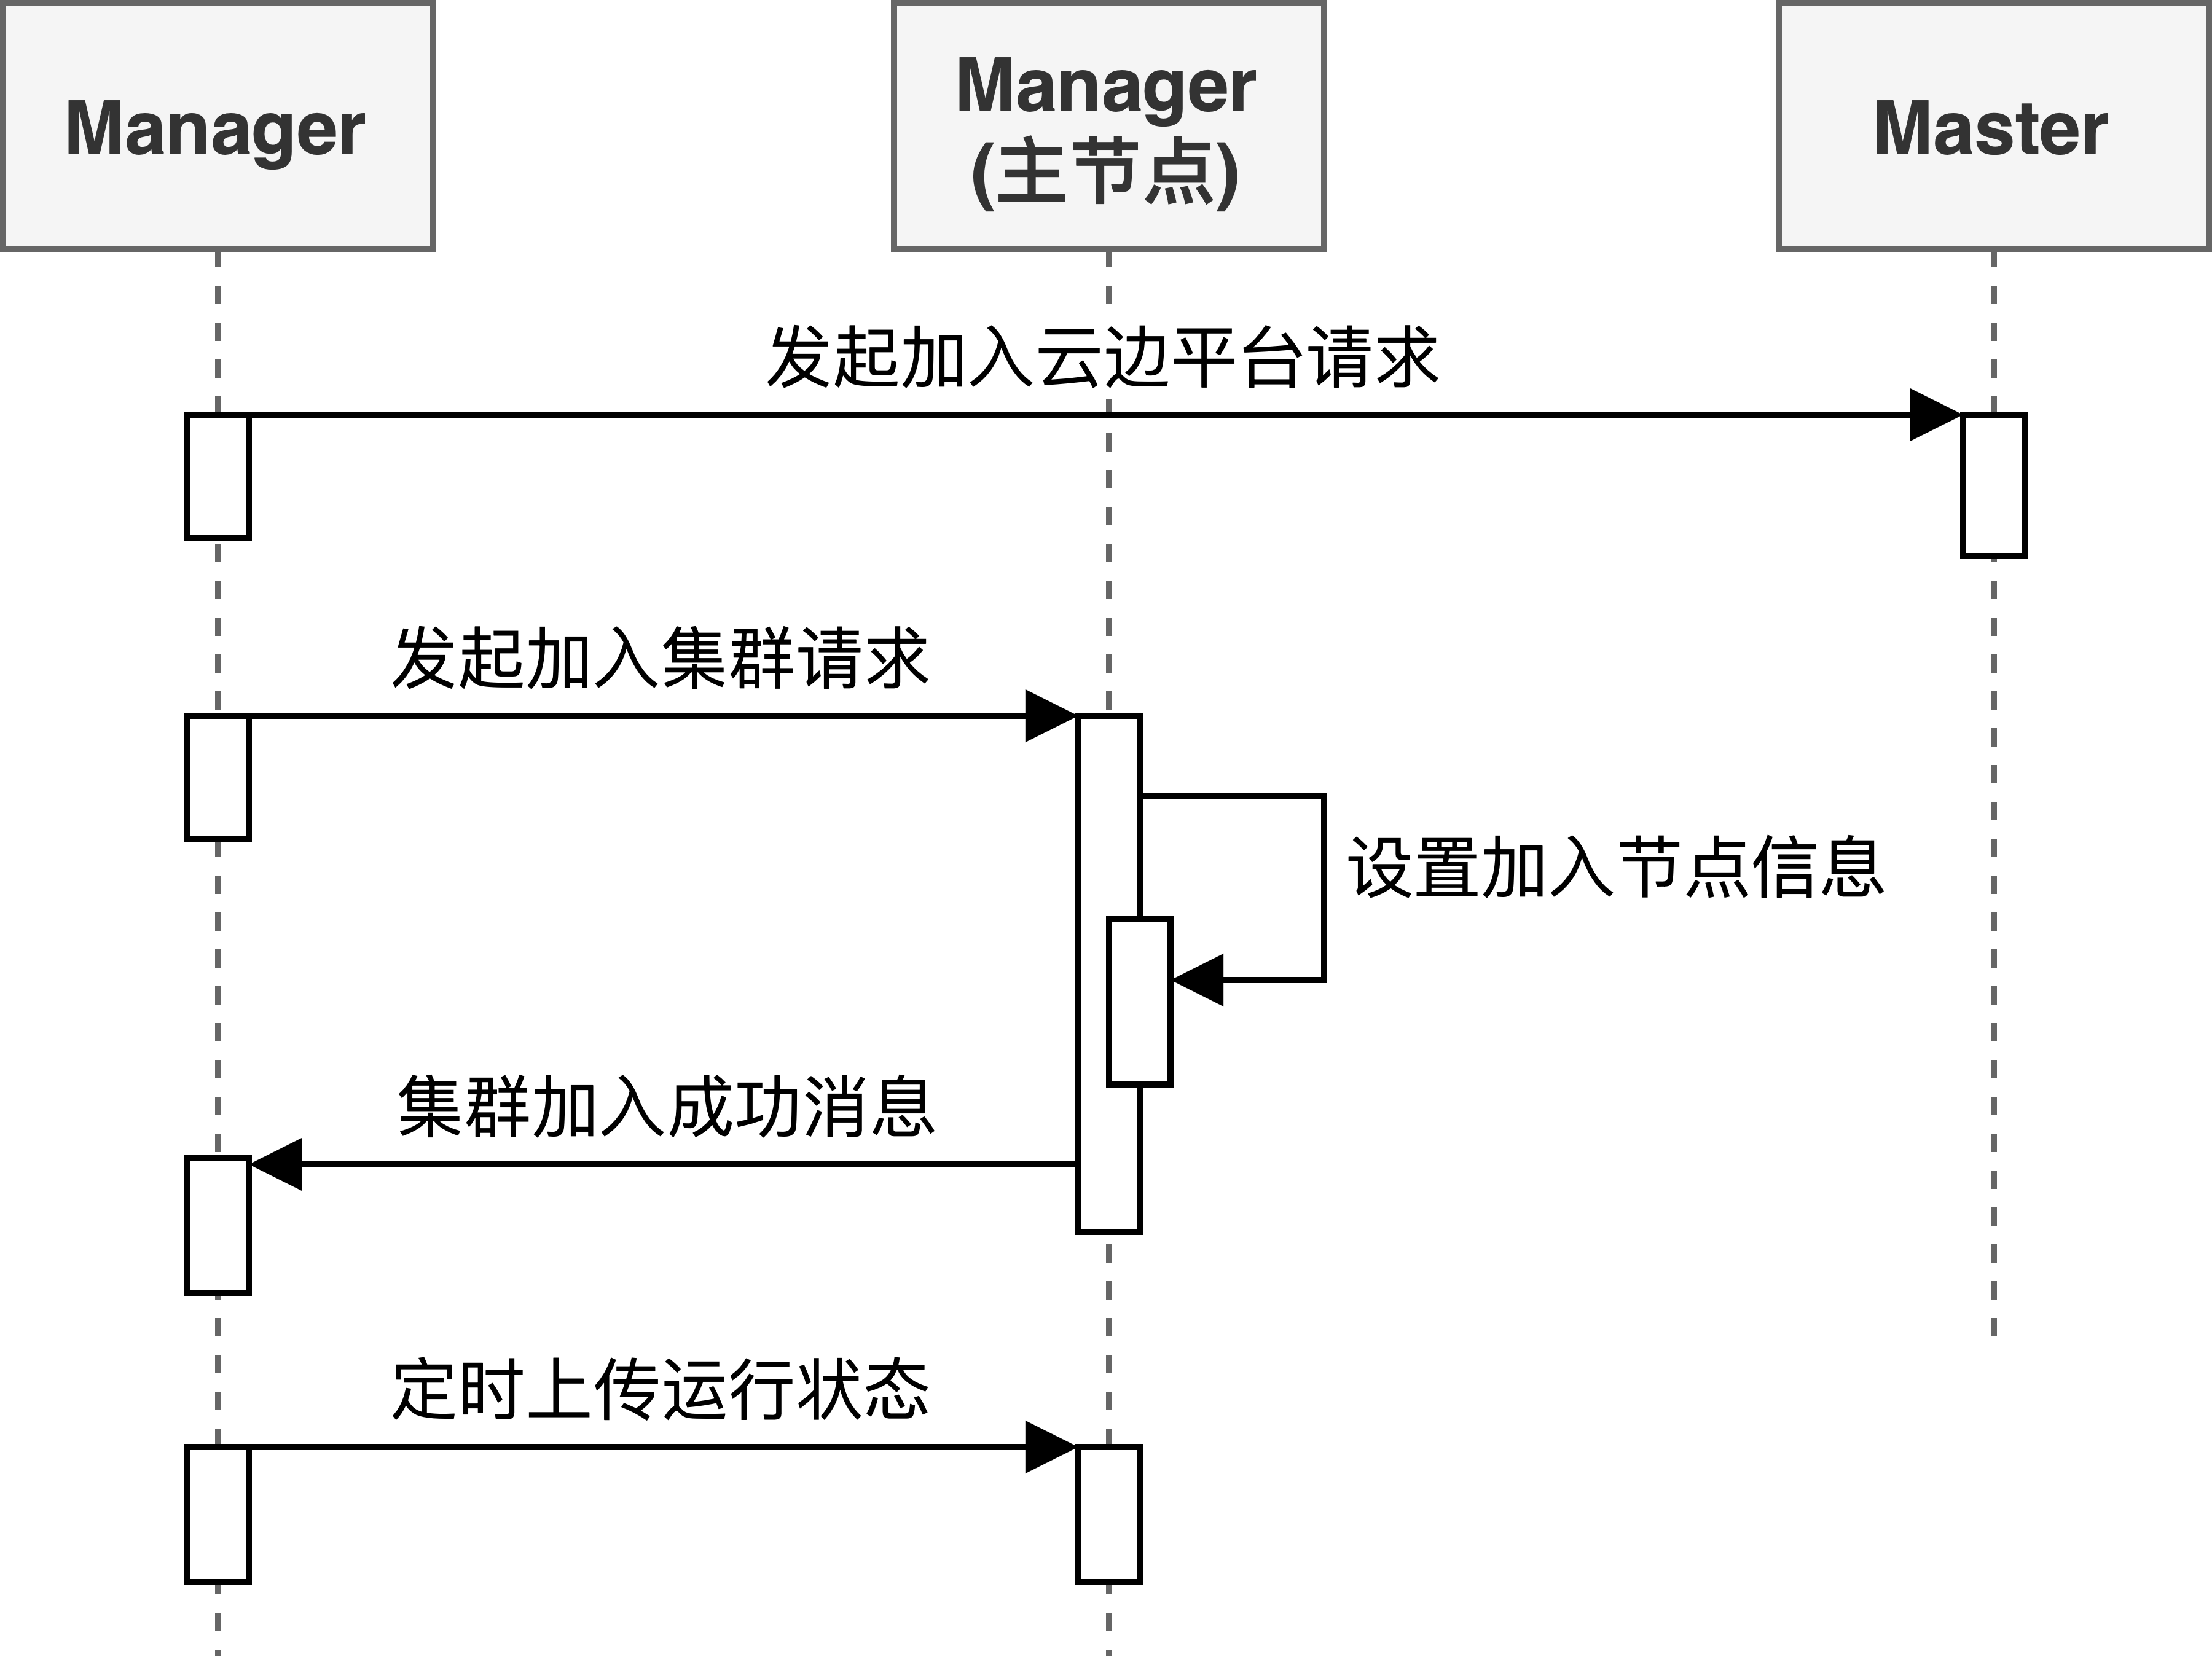
\includegraphics[width=0.7\linewidth]{pics/4-6集群加入.png}
  \caption{新节点加入边缘集群的时序图}
  \label{fig:4-6join}
\end{figure}

边缘管理器(Manager)部署在边缘节点上,主要负责本地任务的调度与资源管理。多个边缘管理器可以组成树状逻辑拓扑结构,每个子树可视为一个边缘集群,其中根节点即为该集群的主节点,承担整个集群的任务调度职责。当有新的边缘节点需要加入集群时,用户需根据实际场景指定一个已属于目标集群的节点作为初始接入点。例如,在实际部署中,用户可以选择与新节点处于同一局域网或同一地理区域的任意一个集群节点作为接入点。如图 \ref{fig:4-6join} 所示,新节点首先通过 Akka Cluster 机制向云端管理器发送加入云边平台的请求。如果用户指定了加入的目标边缘节点,则新节点会向该指定节点发送加入集群的请求消息。这个指定的节点将成为新节点的主节点,并负责配置新节点的相关信息。一旦主节点完成配置,它会返回集群加入成功的消息给新节点。此时,新节点也会设置主节点的信息,并开始定时上报自身的运行状态。

\begin{figure}[ht]
  \centering
  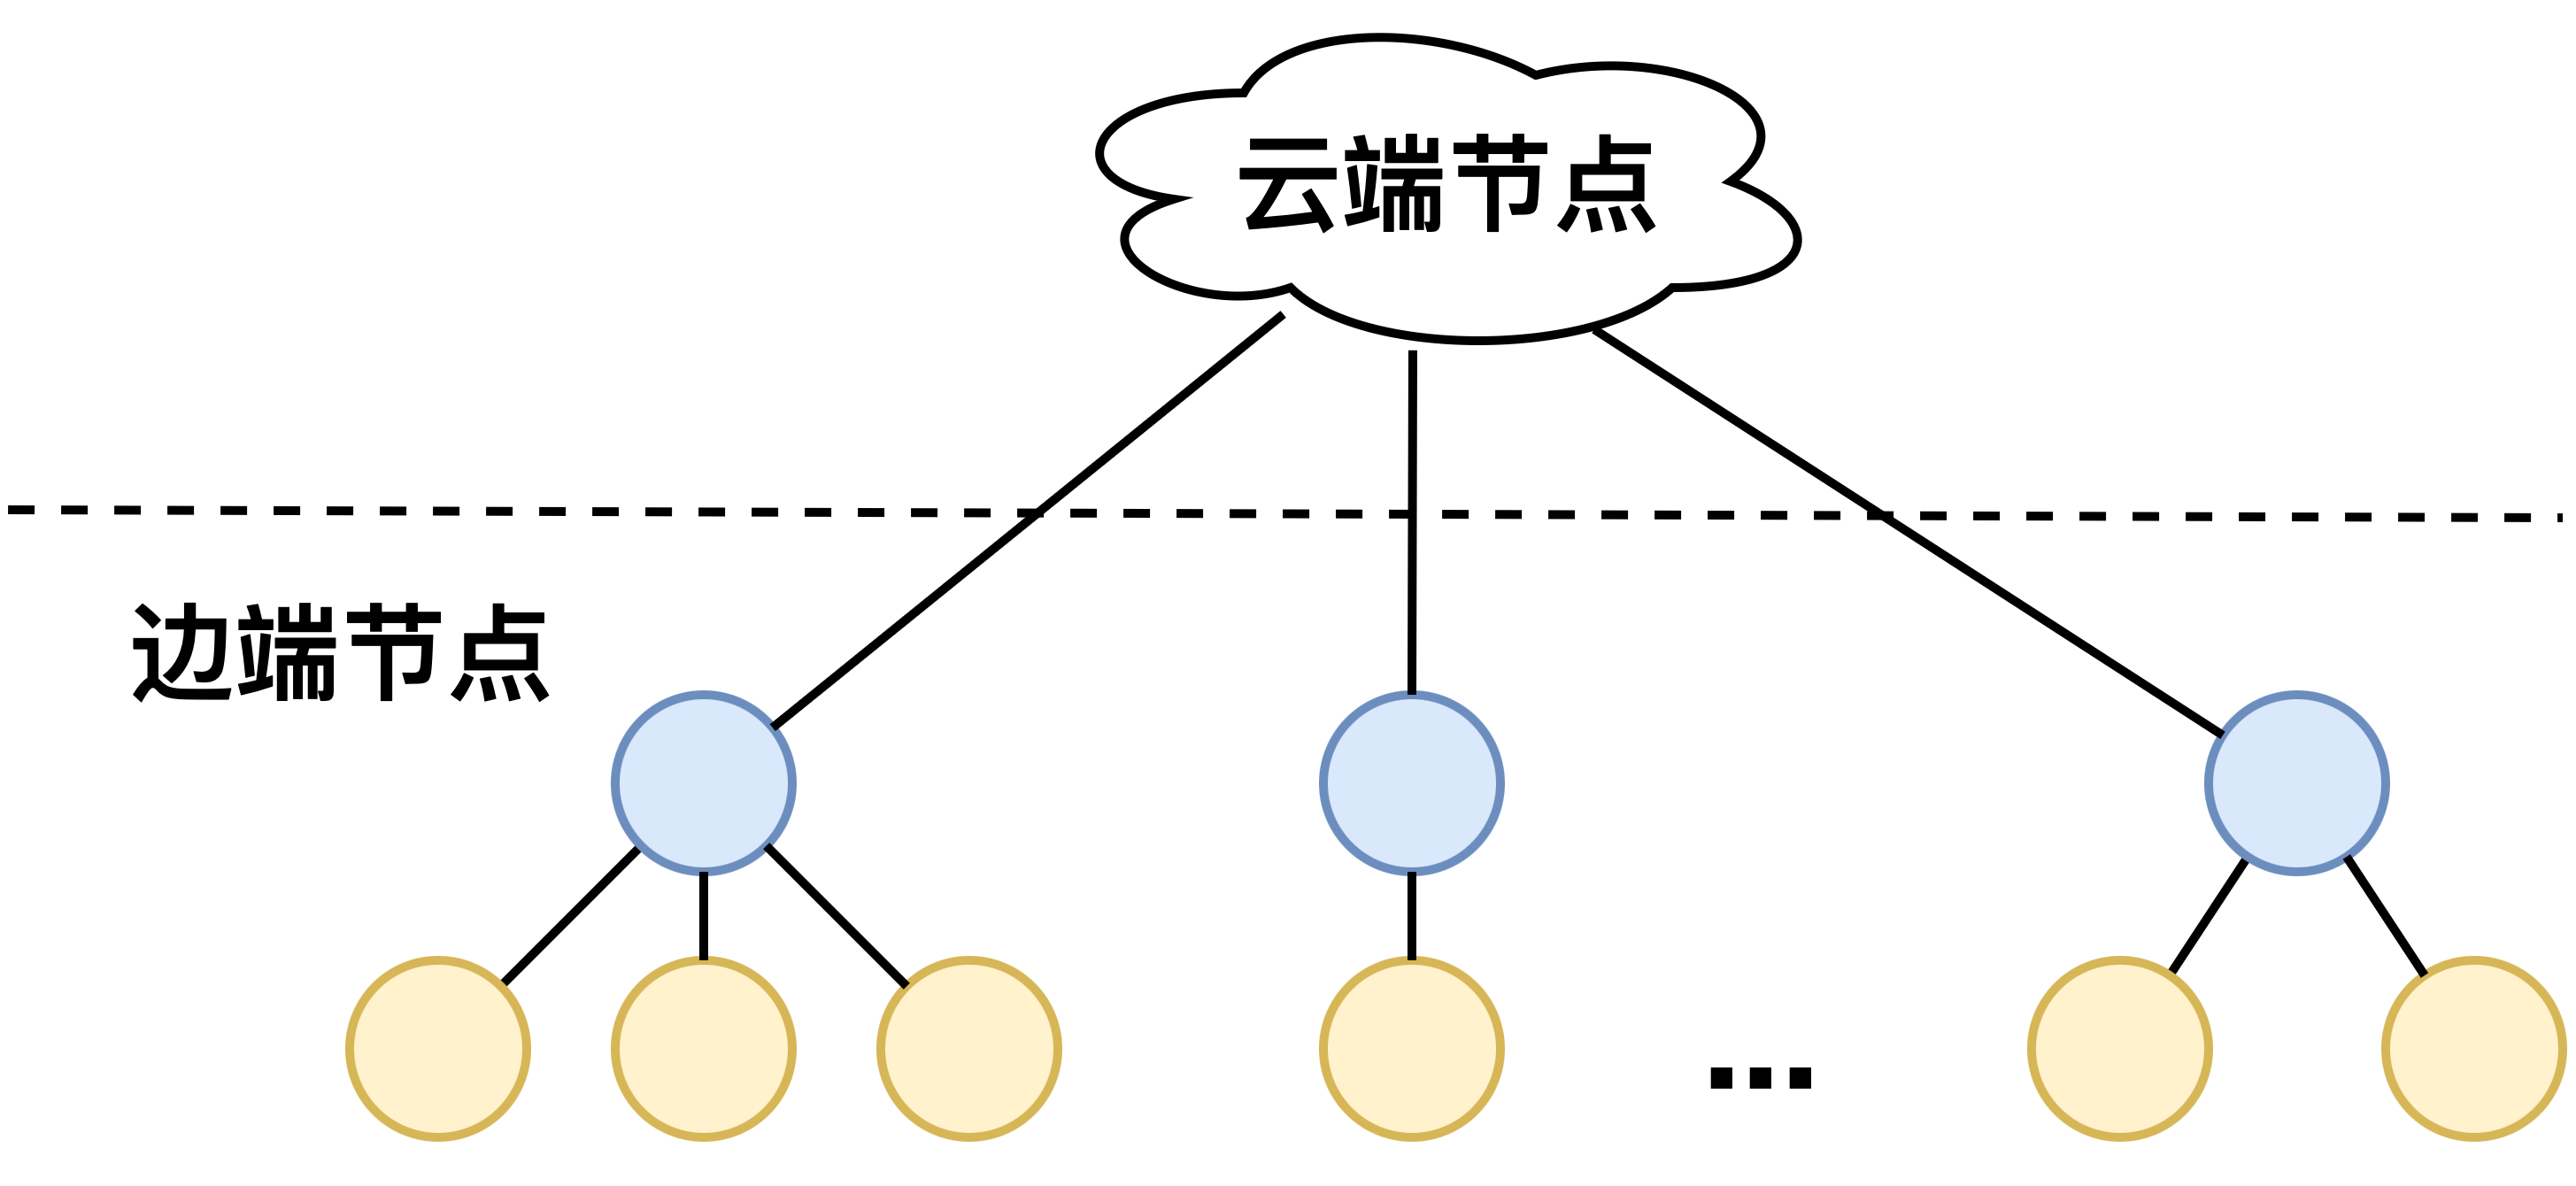
\includegraphics[width=0.6\linewidth]{pics/4-5arc.png}
  \caption{云边拓扑结构}
  \label{fig:4-5arc}
\end{figure}

通过这种方式,本文实现了边缘节点之间的树状逻辑拓扑结构。为了简化论述,本文假设边端节点配置为两层结构,即直接连接设备的节点和集群的主节点,如图 \ref{fig:4-5arc} 所示。这种两层结构不仅便于理解,而且可以轻松扩展到多层结构,当某一层的调度失败时,任务可以自动向上一层进行调度,从而实现高效的资源利用和任务处理。

\subsection{监听协调服务}

本节详细阐述监听协调服务的两大核心功能模块:设备状态监控机制与资源动态部署机制,二者共同构建了云边协同环境下的资源监听与部署能力基础。

\subsubsection{Kubernetes 资源监听机制}

为实现对 Kubernetes 资源的统一监控,监听协调服务通过 Kubernetes 的 Informer 机制与集群通信,实时获取集群的状态信息。对于 Kubernetes 原生资源(如 Pods、Services 等),可直接利用 Kubernetes 提供的内置 Informer 机制完成监控;而对于自定义资源(Custom CRDs),则需独立设计并实现相应的监听模块。为此,本文针对 KubeEdge 的 Device CRDs 设计并实现了专门的监听模块,主要包括两个核心部分:DeviceModel 和 Device,分别用于描述设备的抽象模型与具体实例。

\begin{figure}[ht]
  \centering
  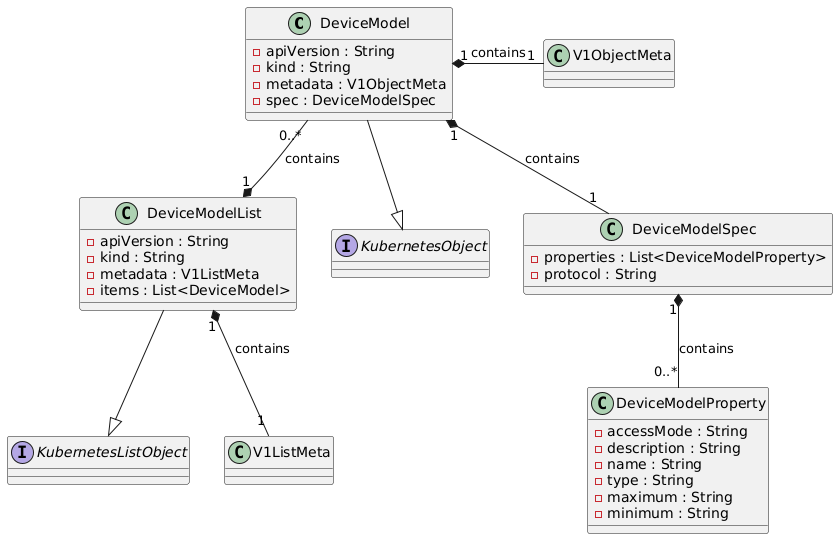
\includegraphics[width=0.95\linewidth]{pics/4-9devicemodel类图.png}
  \caption{DeviceModel 领域层的类图}
  \label{fig:4-9devicemodel}
\end{figure}

图 \ref{fig:4-9devicemodel} 展示了 DeviceModel 领域层的类图。在 KubeEdge 的 Device CRDs 中,DeviceModel 是用于描述设备模型的核心抽象,其设计旨在定义设备的静态属性和协议规范。具体而言,DeviceModel 包含以下关键属性:协议(Protocol)描述设备支持的通信协议及其相关参数;设备模型属性(DeviceModelProperty)表示设备的具体特性,包括属性类型、取值范围以及默认值;属性元数据(Metadata)提供关于设备属性的额外信息,例如访问权限以及更新频率等。

\begin{figure}[ht]
  \centering
  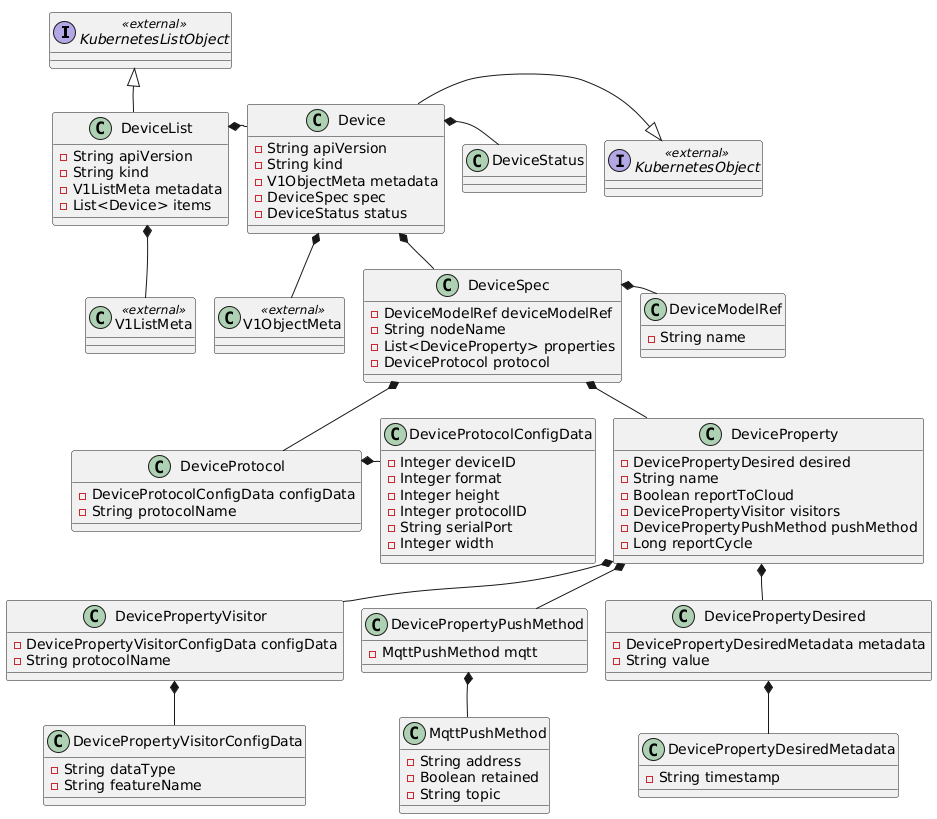
\includegraphics[width=\linewidth]{pics/4-8device类图.png}
  \caption{Device 领域层的类图}
  \label{fig:4-8device}
\end{figure}

图 \ref{fig:4-8device} 展示了 Device 领域层的类图,Device 是用于描述具体设备实例的核心抽象,其设计旨在将物理设备与对应的设备模型关联起来,从而实现从抽象到具体的映射。Device 的核心定义可以分为以下几个部分:设备规格(Spec)通过 deviceModelRef 关联设备元模型,继承设备模型中定义的静态属性和协议规范,同时允许在实例级别通过 properties 属性覆盖设备模型中的默认配置,以满足具体设备的个性化需求;通信协议配置(Protocol)进一步细化了物理设备的通信参数,确保设备与云边协同系统的无缝对接;设备状态(Status)模块则实现了数字孪生体的状态同步,实时记录设备的运行数据与健康状态,为上层应用提供可靠的监控能力。此外,扩展功能模块集成了基于 MQTT 的数据推送策略,通过 reportCycle 字段控制设备数据的上报频率,从而优化网络资源的使用效率。这一设计不仅有效实现了 DeviceModel 中定义的抽象模型,还为实际物理设备的接入与管理提供了灵活且高效的解决方案。

\begin{figure}[ht]
  \centering
  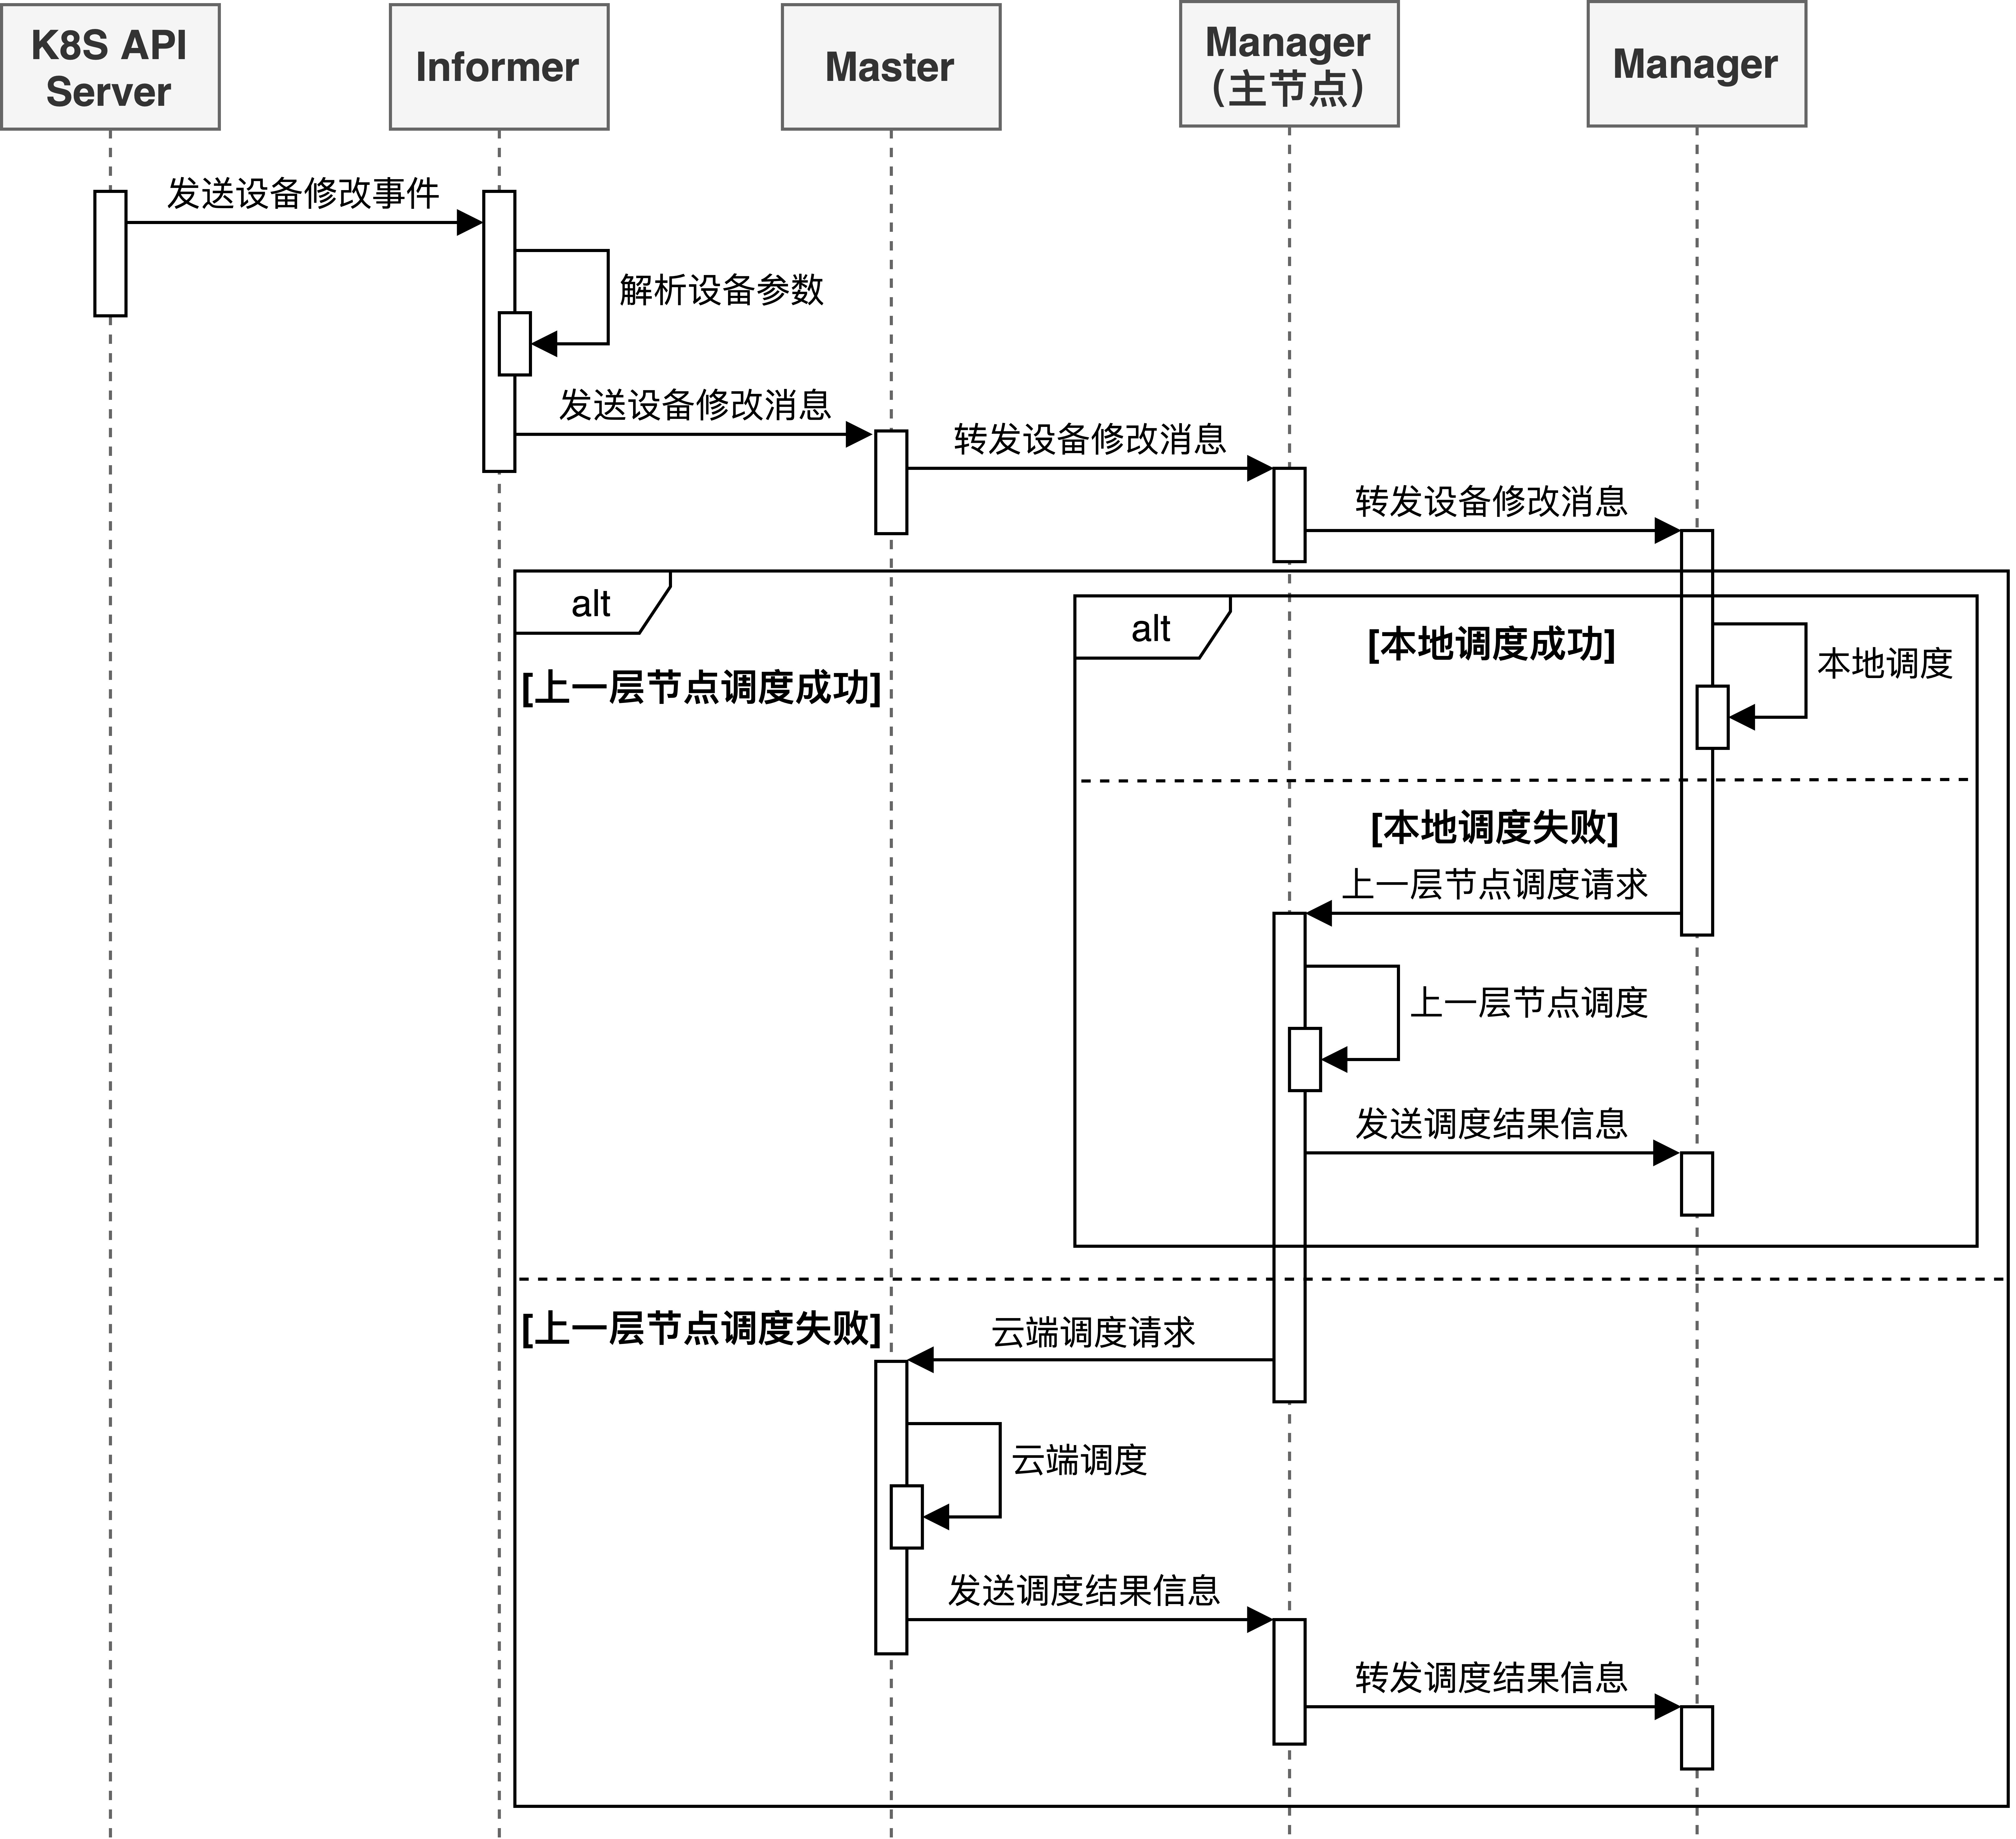
\includegraphics[width=\linewidth]{pics/4-10informer时序.png}
  \caption{基于 Informer 的设备状态监听与调度流程的时序图}
  \label{fig:4-10informer}
\end{figure}

在上述设计的基础上,本文通过 Kubernetes 的 ListAndWatch 方法实现了对设备状态的动态监听。如图\ref{fig:4-10informer}所示,Informer 组件会通过 API Server 提供的长连接机制,实时接收设备信息的变更事件。当设备信息发生变更时,API Server 会主动向客户端推送修改事件,Informer 组件则根据设备的静态信息提取出单次数据采集量和采集频率等关键的变更,并将这些信息封装为 Akka 消息(Message)发送至云端调度器 Master。Master 接收到消息后,将其转发至边缘树状集群主节点 Manager,再由 Manager 将消息分发至设备直连节点的边端管理器,从而触发云边协同环境下的多层次调度机制。设备直连节点的边端管理器会根据设备的变更情况尝试进行本地调度。若本地资源无法满足设备流式数据的需求,则将无法处理的请求转发至上一层节点的边端管理器,触发上一层调度。如果边缘树状集群的资源仍然不足,则进一步将请求转发至云端管理器 Master,由云端完成全局调度。这一多层次的调度机制不仅充分利用了边缘计算的本地化优势,还通过云端的全局视角确保了系统的整体性能与可靠性。

\subsubsection{资源动态部署机制}
\label{sec:deploy-resource}

为满足云边协同系统运行时部署AI模型推理实例等核心负载的需求,本文设计了基于Kubernetes原生资源的资源动态部署机制。该机制通过预置标准化的部署模板,实现了对负载实例的自动化部署。

\begin{figure}[ht]
  \centering
  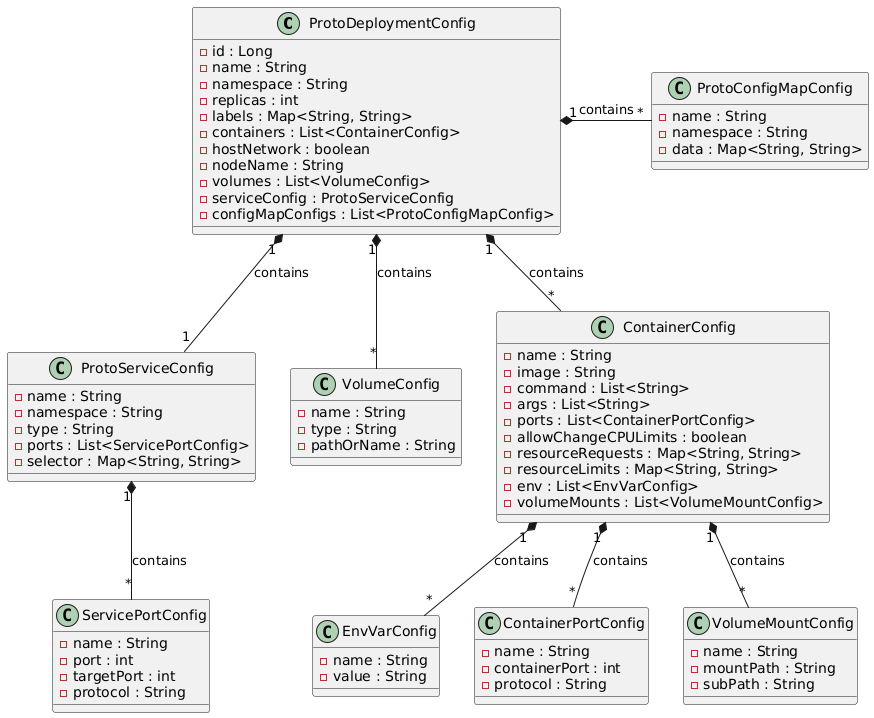
\includegraphics[width=\linewidth]{pics/4-11proto.png}
  \caption{资源动态部署机制的领域层类图}
  \label{fig:4-11proto}
\end{figure}

图 \ref{fig:4-11proto} 展示了资源动态部署机制的领域层类图,核心组件ProtoDeploymentConfig作为配置模板的核心载体,通过组合ProtoServiceConfig和ProtoConfigMapConfig,构建了完整的负载部署配置拓扑。具体而言,ProtoDeploymentConfig以对象图形式封装了Kubernetes Deployment的全部配置参数,包括容器镜像、资源配额、存储卷挂载等运行时属性,并通过ContainerConfig实现对容器启动参数的细粒度控制。当系统调用Kubernetes API时,该配置对象会自动转化为Deployment资源的创建请求,通过API Server完成Pod实例的编排。同时,嵌套的ProtoServiceConfig将通过标签选择器(selector)与Deployment形成语义绑定,确保服务发现机制能够精准路由流量至对应的Pod实例;而ProtoConfigMapConfig则将配置数据以键值对形式注入到Pod中,实现了配置参数的动态更新能力。此外,本设计通过hostNetwork、nodeName等属性实现了对节点亲和性调度的显式控制,并支持HostPath、PersistentVolume等多类型存储卷的挂载配置,使得系统能够灵活适配云边环境中的异构资源约束。这一核心负载原型设计通过领域对象到 Kubernetes 资源的自动化映射机制,将复杂的配置过程封装为标准化接口,使开发人员能够专注于深度学习模型的设计与开发,而无需关心底层部署细节,从而显著降低了云边协同系统的集成复杂度。

\subsection{模型推理服务}

本文的AI模型推理服务专注于推理部署环节。用户需将训练完成的AI模型(包含模型结构与权重)预先上传至对象存储服务,支持MinIO或阿里云等第三方存储方案。本文采用MinIO作为默认存储后端,并通过RESTful API实现模型文件的上传和下载。

\subsubsection{模型推理实例镜像打包}

在工业化的 AI 模型推理领域,现有的成熟框架(如 TensorFlow Serving 和 TorchServe)已经能够通过配置文件挂载预训练模型,实现高效部署推理服务。然而,在云边协同环境中,由于计算节点的异构性问题,这些框架在实际应用中面临诸多挑战。例如,计算节点可能基于不同的硬件架构(如 AMD64、ARMv7 或 ARMv8),并且即使在同一架构下(如 AMD64),也可能存在指令集加速支持的差异(如 AVX2)。为了屏蔽底层硬件差异并减少重复工作,本文为不同架构打包了适配的镜像,如表\ref{tab:multi-arch-images} 所示。具体而言,本文利用 QEMU 模拟多种硬件架构,并结合 Bazel 工具链编译了适配不同架构的 TensorFlow 和 TensorFlow Serving。随后,将编译结果封装为多架构 Docker 镜像,以满足云边协同环境中的多样化需求。在模型部署阶段,系统通过 Kubernetes 的节点标签(Node Labels)机制,根据节点的硬件架构信息动态选择与之匹配的镜像版本,从而确保镜像与目标节点的兼容性。

\begin{table}[ht]
    \renewcommand{\arraystretch}{1.5}
    \centering
    \caption{不同架构的 TensorFlow Serving 镜像}
    \label{tab:multi-arch-images}
    \begin{tabular}{lll}
        \toprule
        \textbf{架构类型} & \textbf{镜像名称} & \textbf{特性说明} \\
        \midrule
        ARM32 (32-bit) & tensorflow-serving:latest-arm32 & 无SIMD加速 \\
        ARM64 (64-bit) & tensorflow-serving:latest-arm64 & NEON指令集优化 \\
        AMD64 & tensorflow-serving:latest-amd64 & 默认支持AVX2加速 \\
        AMD64 (no-AVX2) & tensorflow-serving:noavx2-amd64 & 不依赖AVX2指令集 \\
        \bottomrule
    \end{tabular}
\end{table}

\subsubsection{模型推理实例转换}

尽管 TensorFlow Serving 提供了高效的推理能力,但不同框架训练的模型可能存在兼容性问题。例如,使用 PyTorch 或 Keras 训练的模型无法直接部署到 TensorFlow Serving 中。为此,本文设计了一个微服务模块,用于自动化完成模型的转换与封装。该模块通过解析原始模型文件,将其转换为 ONNX 格式,并生成适配目标推理框架的配置文件,从而简化了跨框架部署的复杂性。该模块的生命周期如图\ref{fig:4-12trans}所示,主要包括创建状态、下载状态、模型转换状态、上传模型状态、失败状态和结束状态,各状态间的转换遵循严格的工作流控制机制,具体如下:

\begin{figure}[ht]
  \centering
  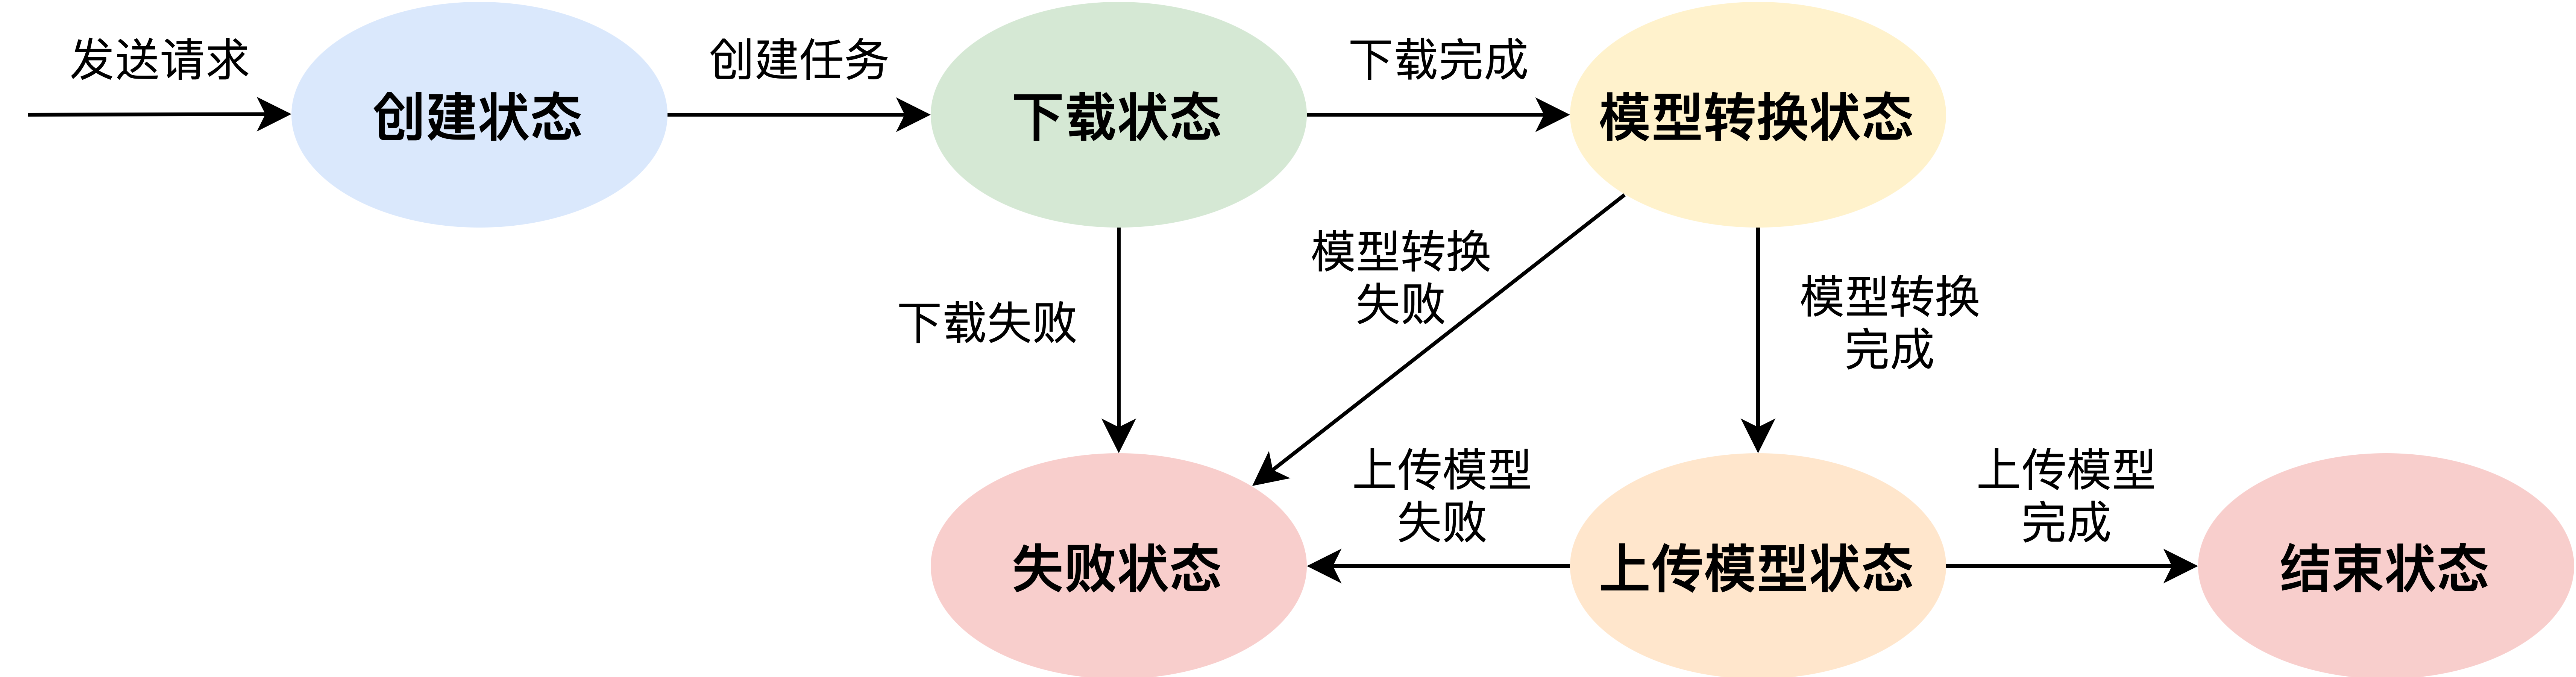
\includegraphics[width=\linewidth]{pics/4-12模型转换.png}
  \caption{AI模型转换模块的生命周期}
  \label{fig:4-12trans}
\end{figure}

\begin{itemize}
    \item \textbf{创建状态:} 系统接收转换请求后,首先验证输入参数的有效性,包括源模型路径、目标格式兼容性以及 MinIO 存储连接状态。验证通过后,系统生成唯一任务标识符并创建任务记录,并客户端返回任务 ID,同时启动异步模型转换流程。
    \item \textbf{下载状态:} 进入异步下载处理后,系统首先在临时存储中建立隔离的工作目录结构,然后从 MinIO 对象存储获取源模型。此阶段支持多种模型存储形式,包括单文件模型、目录结构模型(如 TensorFlow SavedModel)以及压缩包模型。若源模型为压缩格式,系统会自动解压并识别其中的有效模型文件。下载过程中如遇网络故障或权限问题,任务将直接转入失败状态。
    \item \textbf{模型转换状态:} 模型下载完成后,系统根据源格式和目标格式确定转换路径。首先将源模型转换为 ONNX 中间表示,再从 ONNX 转换为目标格式。转换过程保留计算图结构、权重参数和输入输出规格,同时执行模型验证以确保转换精度达到预期要求。
    \item \textbf{上传模型状态:} 模型成功转换后,系统将结果模型打包并上传至用户指定的 MinIO 存储位置。此阶段会自动处理不同模型格式的特殊要求,例如将目录结构模型压缩为 ZIP 文件,或者将大型模型分片上传以提高传输可靠性。
    \item \textbf{失败和结束状态:} 整个生命周期中的任何阶段出现异常,均会触发失败状态转换。对于不同类型的失败,系统应用了差异化的恢复策略,例如网络故障会触发重试机制,而格式不兼容则直接标记为永久性失败。无论成功还是失败,系统最终都会清理临时资源,确保服务器资源得到有效释放。
\end{itemize}

\subsubsection{模型推理实例动态部署}

\begin{figure}[ht]
  \centering
  \includegraphics[width=\linewidth]{pics/4-13deployai.png}
  \caption{模型推理实例部署的时序图}
  \label{fig:4-13deployai}
\end{figure}

结合上述模型推理实例镜像打包、模型推理实例转换模块以及 \ref{sec:deploy-resource} 小节中描述的资源动态部署机制,可以实现模型推理实例动态部署流程。如图 \ref{fig:4-13deployai} 所示,当用户通过 HTTP 请求发起模型推理实例部署请求时,系统内置的控制器(Controller)会捕获该请求并将其转发至云端管理器(Master)。云端管理器在接收到请求后,会创建一个专门负责部署任务的 Actor(Deploy Actor),并将与部署相关的完整上下文信息传递给该 Actor,以驱动后续的部署流程。Deploy Actor 首先解析目标模型的框架类型。若检测到目标推理引擎与模型框架之间存在兼容性问题,则触发模型转换流程,调用模型转换模块完成格式适配。随后,Deploy Actor 会轮询确认模型转换的成功状态,并从 MinIO 存储中获取模型文件的存储地址。该地址通过边缘集群主节点被转发至目标部署节点,目标节点则从 MinIO 下载模型文件并完成解压等预处理操作。在此基础上,Deploy Actor 根据节点加入时由 Informer 提供的节点架构信息,结合资源动态部署机制生成适配目标节点资源环境的核心部署配置。最终,Deploy Actor 通过 Kubernetes API Server 创建相应的 Deployment 和 Service 等资源对象,从而完成整个部署流程。

\subsubsection{模型推理实例批处理测试}

当模型推理实例部署到节点后,若该模型支持批处理(batch processing),系统会触发批处理测试以评估模型在目标节点上的性能表现并确定最优的批处理规模(batch size)。如图\ref{fig:4-14batch}所示,批处理测试分为两个阶段:初始快速上升阶段和精细化搜索阶段。在快速上升阶段,系统以$2^n$次方指数增长的方式逐步增加批处理规模,直至出现资源过载(如内存溢出OOM、CPU/GPU使用率饱和等)为止。此时,系统确认查找范围并进入精细化搜索阶段,采用二分法逐步缩小批处理规模,直至找到系统可承受的最大批处理值。在此过程中,系统同时记录每个批处理规模下的平均数据处理时间,并以最小化单个数据的平均处理时间为优化目标。需要注意的是,虽然批处理通常能够显著降低单位数据的推理开销,但过大的批处理规模可能导致资源竞争加剧,反而降低整体性能。

\begin{algorithm}[ht]
\caption{批处理规模优化测试算法}
\label{alg:batch_size_optimization_simple}
\begin{algorithmic}[1]
\REQUIRE 模型 $Model$, 输入样例 $Input$, 初始批量 $B_{init}$
\ENSURE 最优批处理大小 $B_{opt}$, 最优单数据平均处理时间 $t_{avg\_opt}$

\STATE Initialize $B_{max} \leftarrow 0$, $t_{avg\_opt} \leftarrow \infty$, $B_{opt} \leftarrow 0$

\STATE $B \leftarrow B_{init}$
\WHILE{$B$ succeeds}
  \STATE $(t_{total}, t_{avg}) \leftarrow$ GetTime($B$)
  \STATE $B_{max} \leftarrow B$
  \IF{$t_{avg} < t_{avg\_opt}$}
    \STATE $t_{avg\_opt} \leftarrow t_{avg}$, $B_{opt} \leftarrow B$
  \ELSIF{$t_{avg} > t_{avg\_opt}$} 
    \STATE break \COMMENT{提前终止搜索,避免无效的更大批量}
  \ENDIF
  \STATE $B \leftarrow B \times 2$ \COMMENT{批处理大小加倍}
\ENDWHILE
\STATE $lower \leftarrow B_{max}$, $upper \leftarrow B$ \COMMENT{$B$是首次失败或性能变差的批量}
\WHILE{$lower < upper - 1$}
  \STATE $B_{mid} \leftarrow \lfloor(lower + upper) / 2\rfloor$
  \IF{$B_{mid}$ succeeds}
    \STATE $(t_{total}, t_{avg}) \leftarrow$ GetTime($B_{mid}$)
    \STATE $lower \leftarrow B_{mid}$
    \IF{$t_{avg} < t_{avg\_opt}$}
      \STATE $t_{avg\_opt} \leftarrow t_{avg}$, $B_{opt} \leftarrow B_{mid}$
    \ENDIF
  \ELSE
    \STATE $upper \leftarrow B_{mid}$
  \ENDIF
\ENDWHILE

\RETURN $B_{opt}$, $t_{avg\_opt}$
\end{algorithmic}
\end{algorithm}

具体的算法如算法\ref{alg:batch_size_optimization_simple}所示。该算法的时间复杂度主要由两部分组成:第一阶段的指数增长搜索复杂度为 $O(\log B_{max})$,其中 $B_{max}$ 是系统能承受的最大批量;第二阶段的二分查找复杂度为 $O(\log(B - B_{max}))$,因此总复杂度为 $O(\log B_{max} + \log(B - B_{max}))$,整体表现为高效的对数级复杂度。在完成批处理规模优化测试后,系统会根据算法\ref{alg:batch_size_optimization_simple}确定的最优批处理大小 $B_{opt}$ 配置 TensorFlow Serving 的批处理参数。

\begin{figure}[ht]
  \centering
  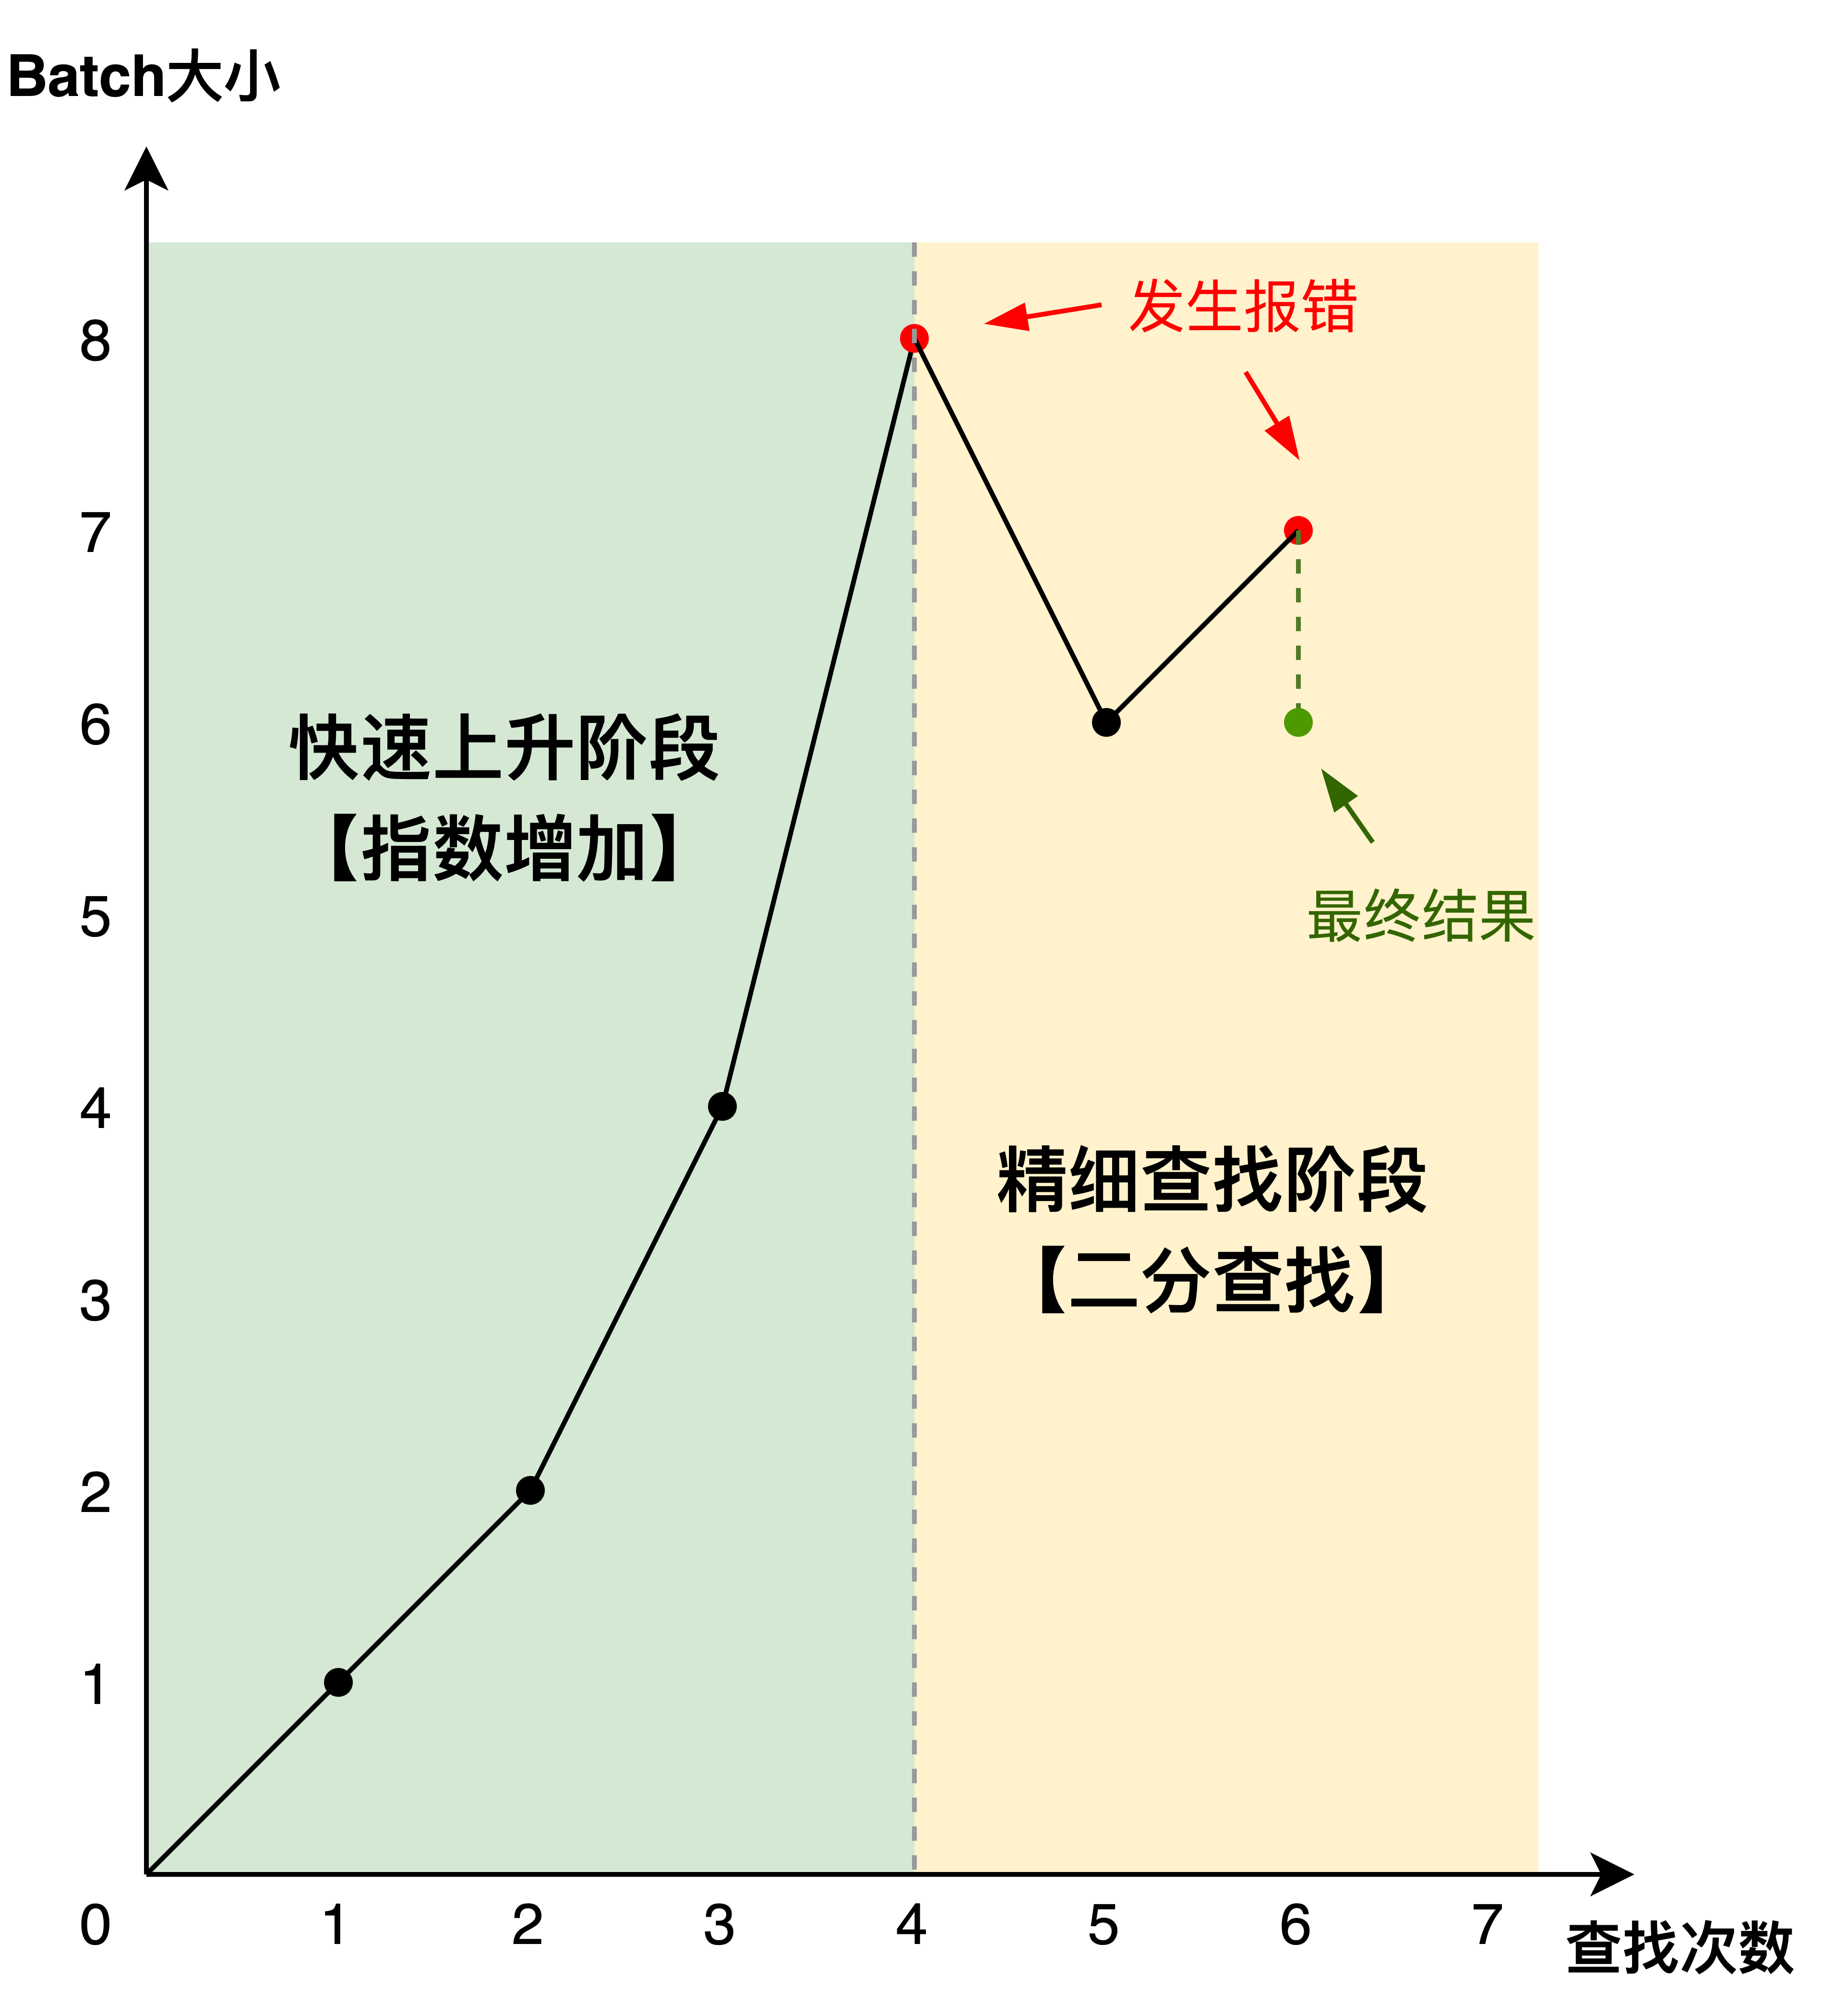
\includegraphics[width=0.6\linewidth]{pics/4-14批查找过程.png}
  \caption{模型推理实例批处理规模优化}
  \label{fig:4-14batch}
\end{figure}

\subsection{数据路由服务}

数据路由服务是KEAS系统中实现高效数据分发与处理的核心组件。该服务通过多个子 Actor 的协同工作完成复杂的任务调度与数据流转。这些子 Actor 由边缘管理器(Manager)动态创建和管理,主要负责订阅设备的流式数据、执行数据转发,并与本地模型推理服务模块进行交互。如图\ref{fig:data-routing-architecture}所示,边缘管理器(Manager)根据云端管理器(Master)下发的全局路由表、或边缘集群生成的集群内部路由表,或本地生成的本地路由表,初始化一条包含订阅 Actor(Sub Actor)和路由 Actor(Router Actor)等核心组件的执行链。在数据采集阶段,Sub Actor 借助 Akka Streams 工具包连接 MQTT 消息代理(如 Mosquitto),以订阅来自设备的实时流式数据。随后,在数据分发阶段,Sub Actor 将接收到的数据及其对应的路由信息转发至 Router Actor。Router Actor 根据路由规则对数据流向进行决策:对于需要跨节点协作的数据,将其转发至其他节点的消息代理;对于需要本地处理的数据,则将其传递给本地的模型推理模块。最后,在数据处理阶段,模型推理服务模块对接收到的数据进行预处理,并将其整理为适合批处理的形式。经过预处理的数据通过 HTTP 或 gRPC 协议发送至模型推理实例,从而完成推理任务。

\begin{figure}[ht]
  \centering
  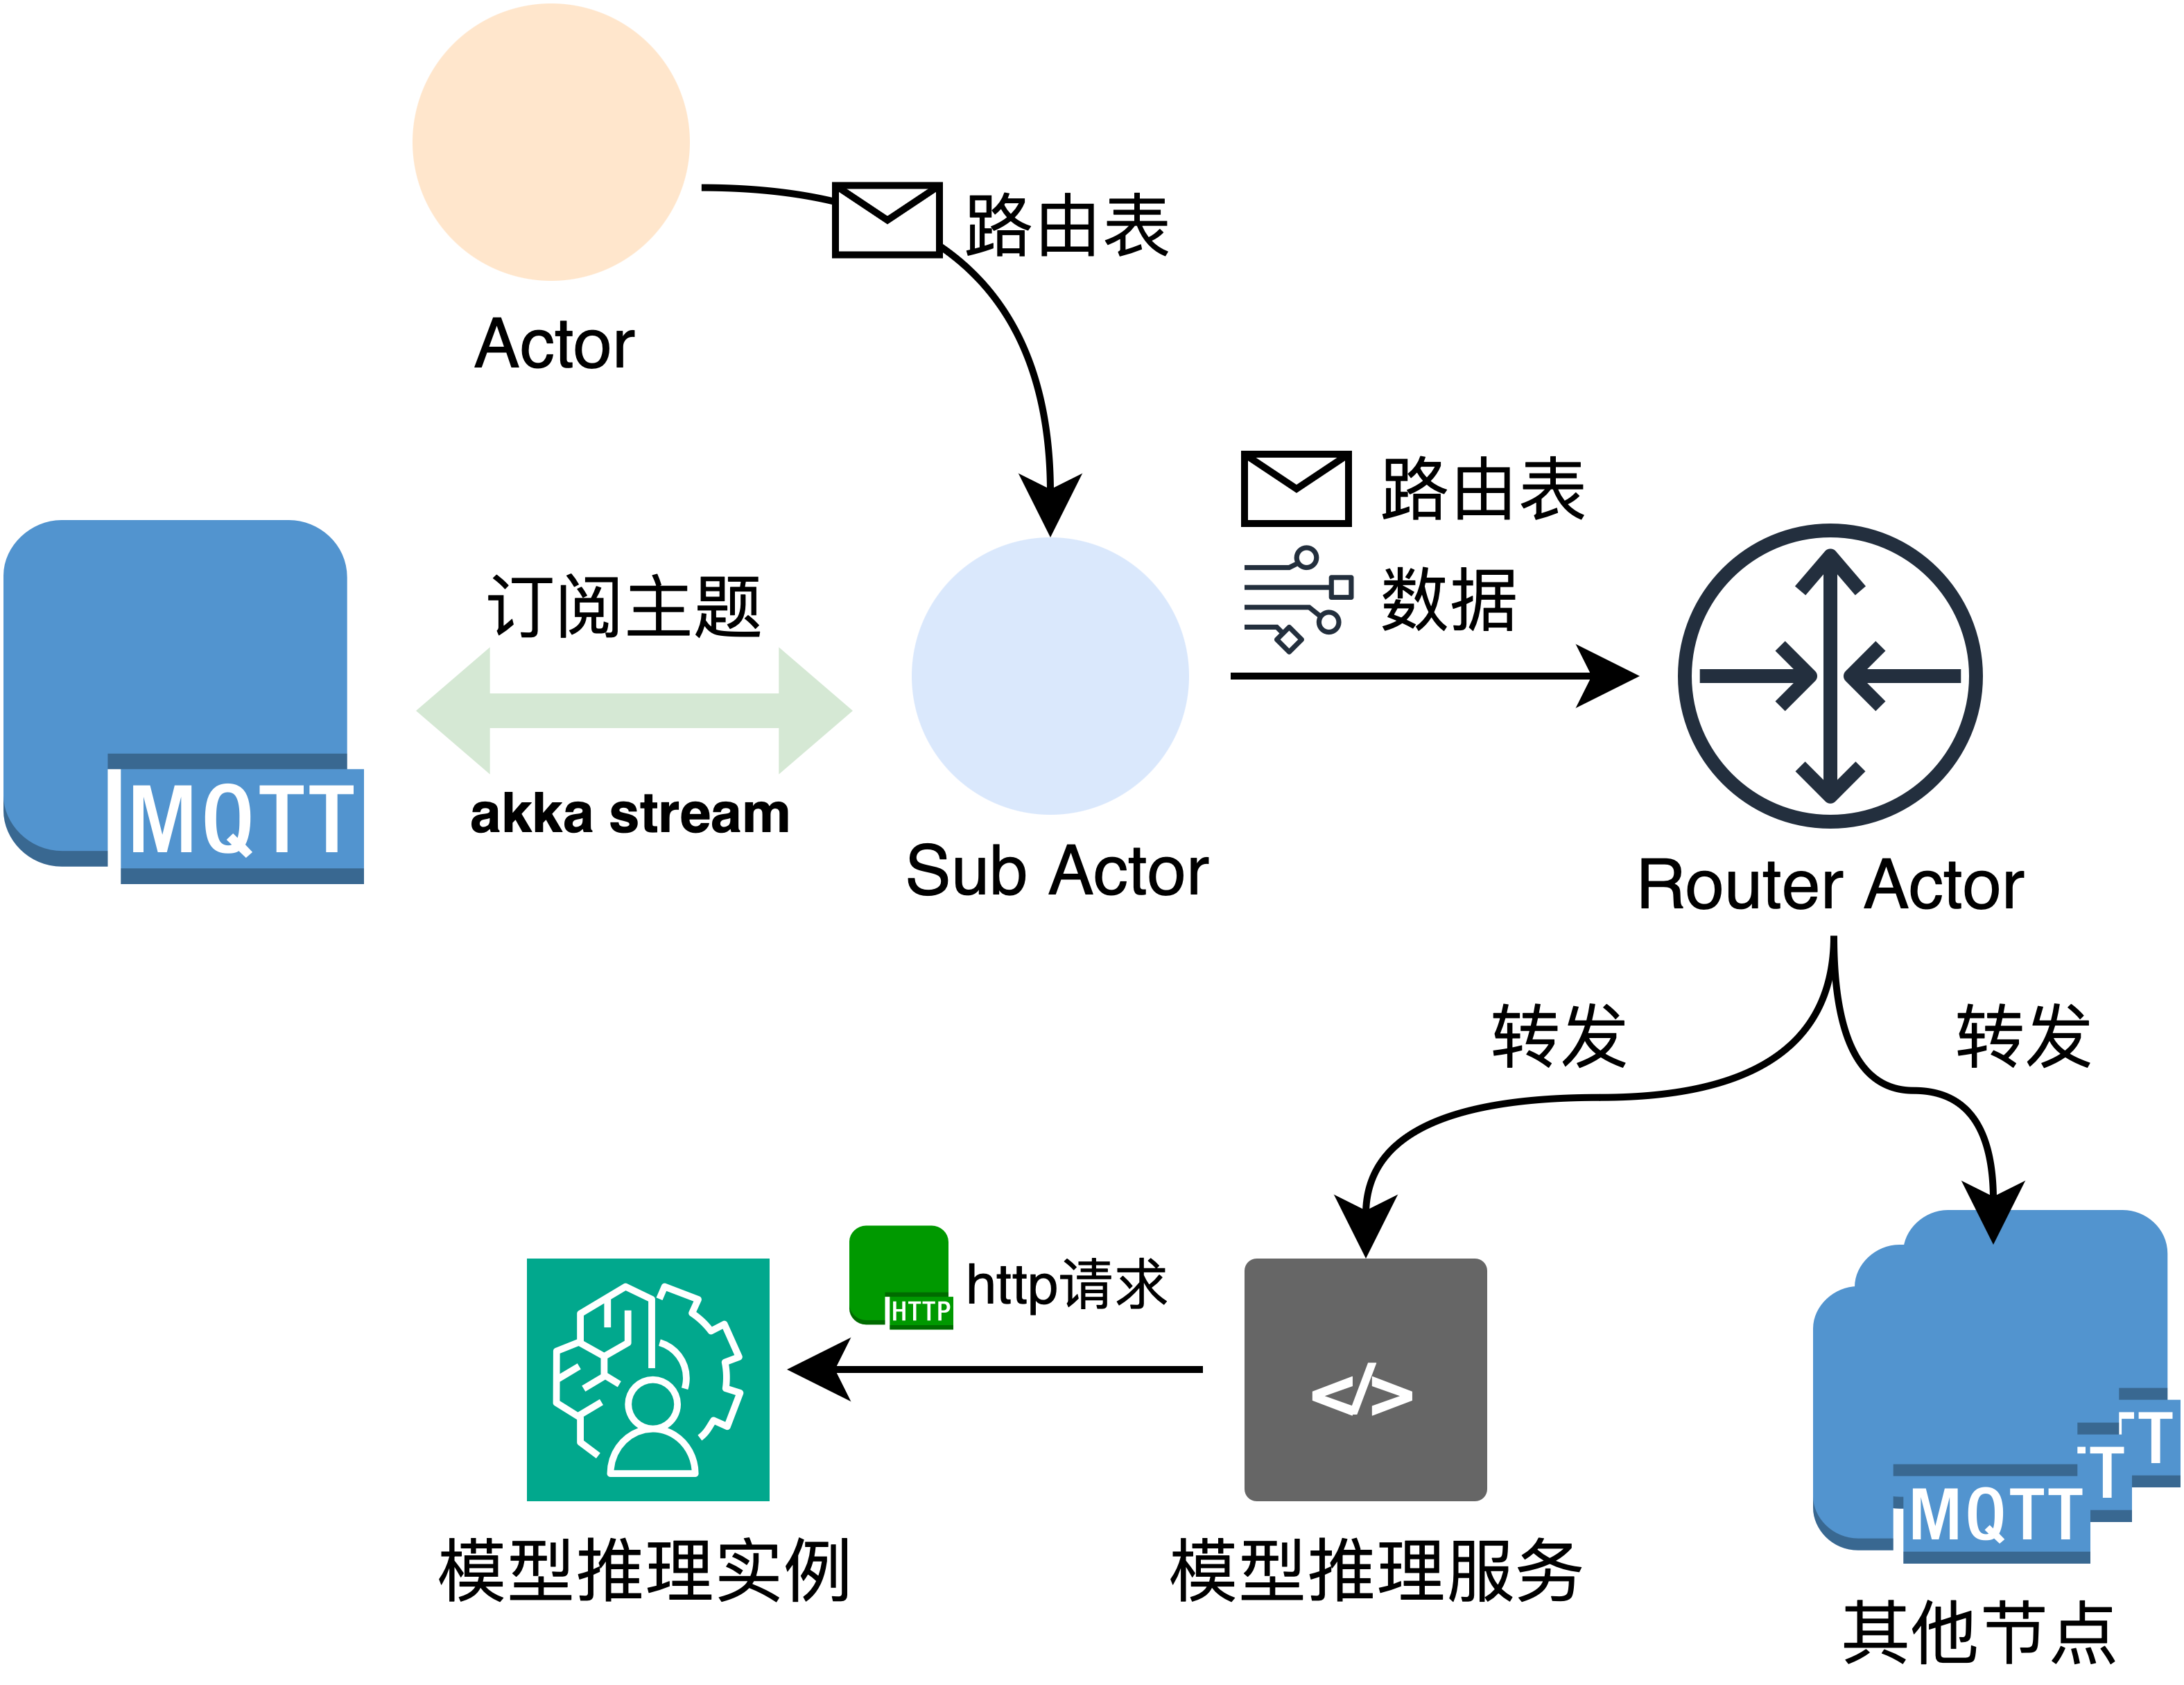
\includegraphics[width=0.75\linewidth]{pics/4-6worker.png}
  \caption{数据流路由服务架构}
  \label{fig:data-routing-architecture}
\end{figure}

此外,Router Actor 会持续监控模型推理服务模块的运行速度,并定期将相关性能指标上报给本地的边缘管理器,以实现运行状态的实时监控。这些监控数据首先被用于本地优化;随后,这些数据会被上传至上一层节点,为上一层节点的资源调度和负载均衡提供依据;同时,边缘树状集群主节点会进一步汇总这些数据并上传至云端,从而支持全局范围内的资源调度、性能分析以及长期趋势预测。

\subsection{系统监控服务}

系统监控服务不仅涵盖上一小节提到的对模型推理服务模块运行速度和任务队列状态的监控,还包括对云边环境下网络状况的全面监测,以确保调度决策的高效性与准确性。最终,所有监控数据将被汇总至 Prometheus,并通过 Grafana 进行可视化展示。

\subsubsection{网络监控探针}

本文采用主被动结合的混合监测方案,构建多维度网络性能评估体系。主动监测模块通过模拟网络流量直接测量关键性能指标,被动监测模块基于实际业务流量分析间接推断网络状态,二者共同覆盖端到端时延、带宽利用率、丢包率等核心维度,为云边协同环境中的资源调度与优化提供全面数据支撑。

主动监测模块通过可控的测试流量直接测量节点间的网络性能指标,主要包括端到端时延和带宽利用率两个方面。端到端时延测量利用 Ping 工具实现,系统定时发送探测请求并根据往返时间(RTT)计算网络延迟。为减少噪声干扰并提高数据稳定性,本文采用指数加权移动平均算法对时延数据进行平滑处理,其公式定义为:
为减少噪声干扰并提高数据稳定性,本文采用指数加权移动平均算法对时延数据进行平滑处理,其公式定义为:
\[
S_t = \alpha X_t + (1-\alpha)S_{t-1},
\]
其中,$S_t$ 表示当前时刻的平滑值,$X_t$ 为原始观测值,$\alpha \in (0,1]$ 为平滑系数,用于控制历史数据与当前观测值的权重分配。带宽测量采用 iPerf3 工具实现,通过动态调整 TCP 窗口大小与数据包分片策略,分别获取单向与双向带宽指标。此外,探测周期根据边缘节点的实时负载智能调整:在空闲时段采用短周期以实现快速响应,在高负载时段切换至长周期,从而在保证测量精度的同时降低系统开销,确保资源占用与性能需求之间的平衡。

被动监测模块基于实际业务流量的行为特征,通过分析节点间的通信数据间接推断网络性能。Node Exporter 是实现被动监测的核心工具,能够实时采集节点网卡的流量统计信息,包括接收/发送字节数、丢包率、错误率等关键指标。通过对单位时间内流量变化的分析,可以估算节点间的实际带宽利用率,并捕捉网络链路的拥塞状态。此外,基于 Node Exporter 采集的流量数据,结合历史记录和统计模型,可以间接估算节点间的网络时延。例如,通过分析数据包到达时间间隔及其分布特征,可以推断出网络延迟的大致范围。尽管被动监测方法的精度略低于主动测量,但其无需额外的探测流量,适合在高负载或受限环境中使用,从而为系统的整体性能评估提供了补充视角。

\subsubsection{监控汇总模块}

\begin{figure}[ht]
  \centering
  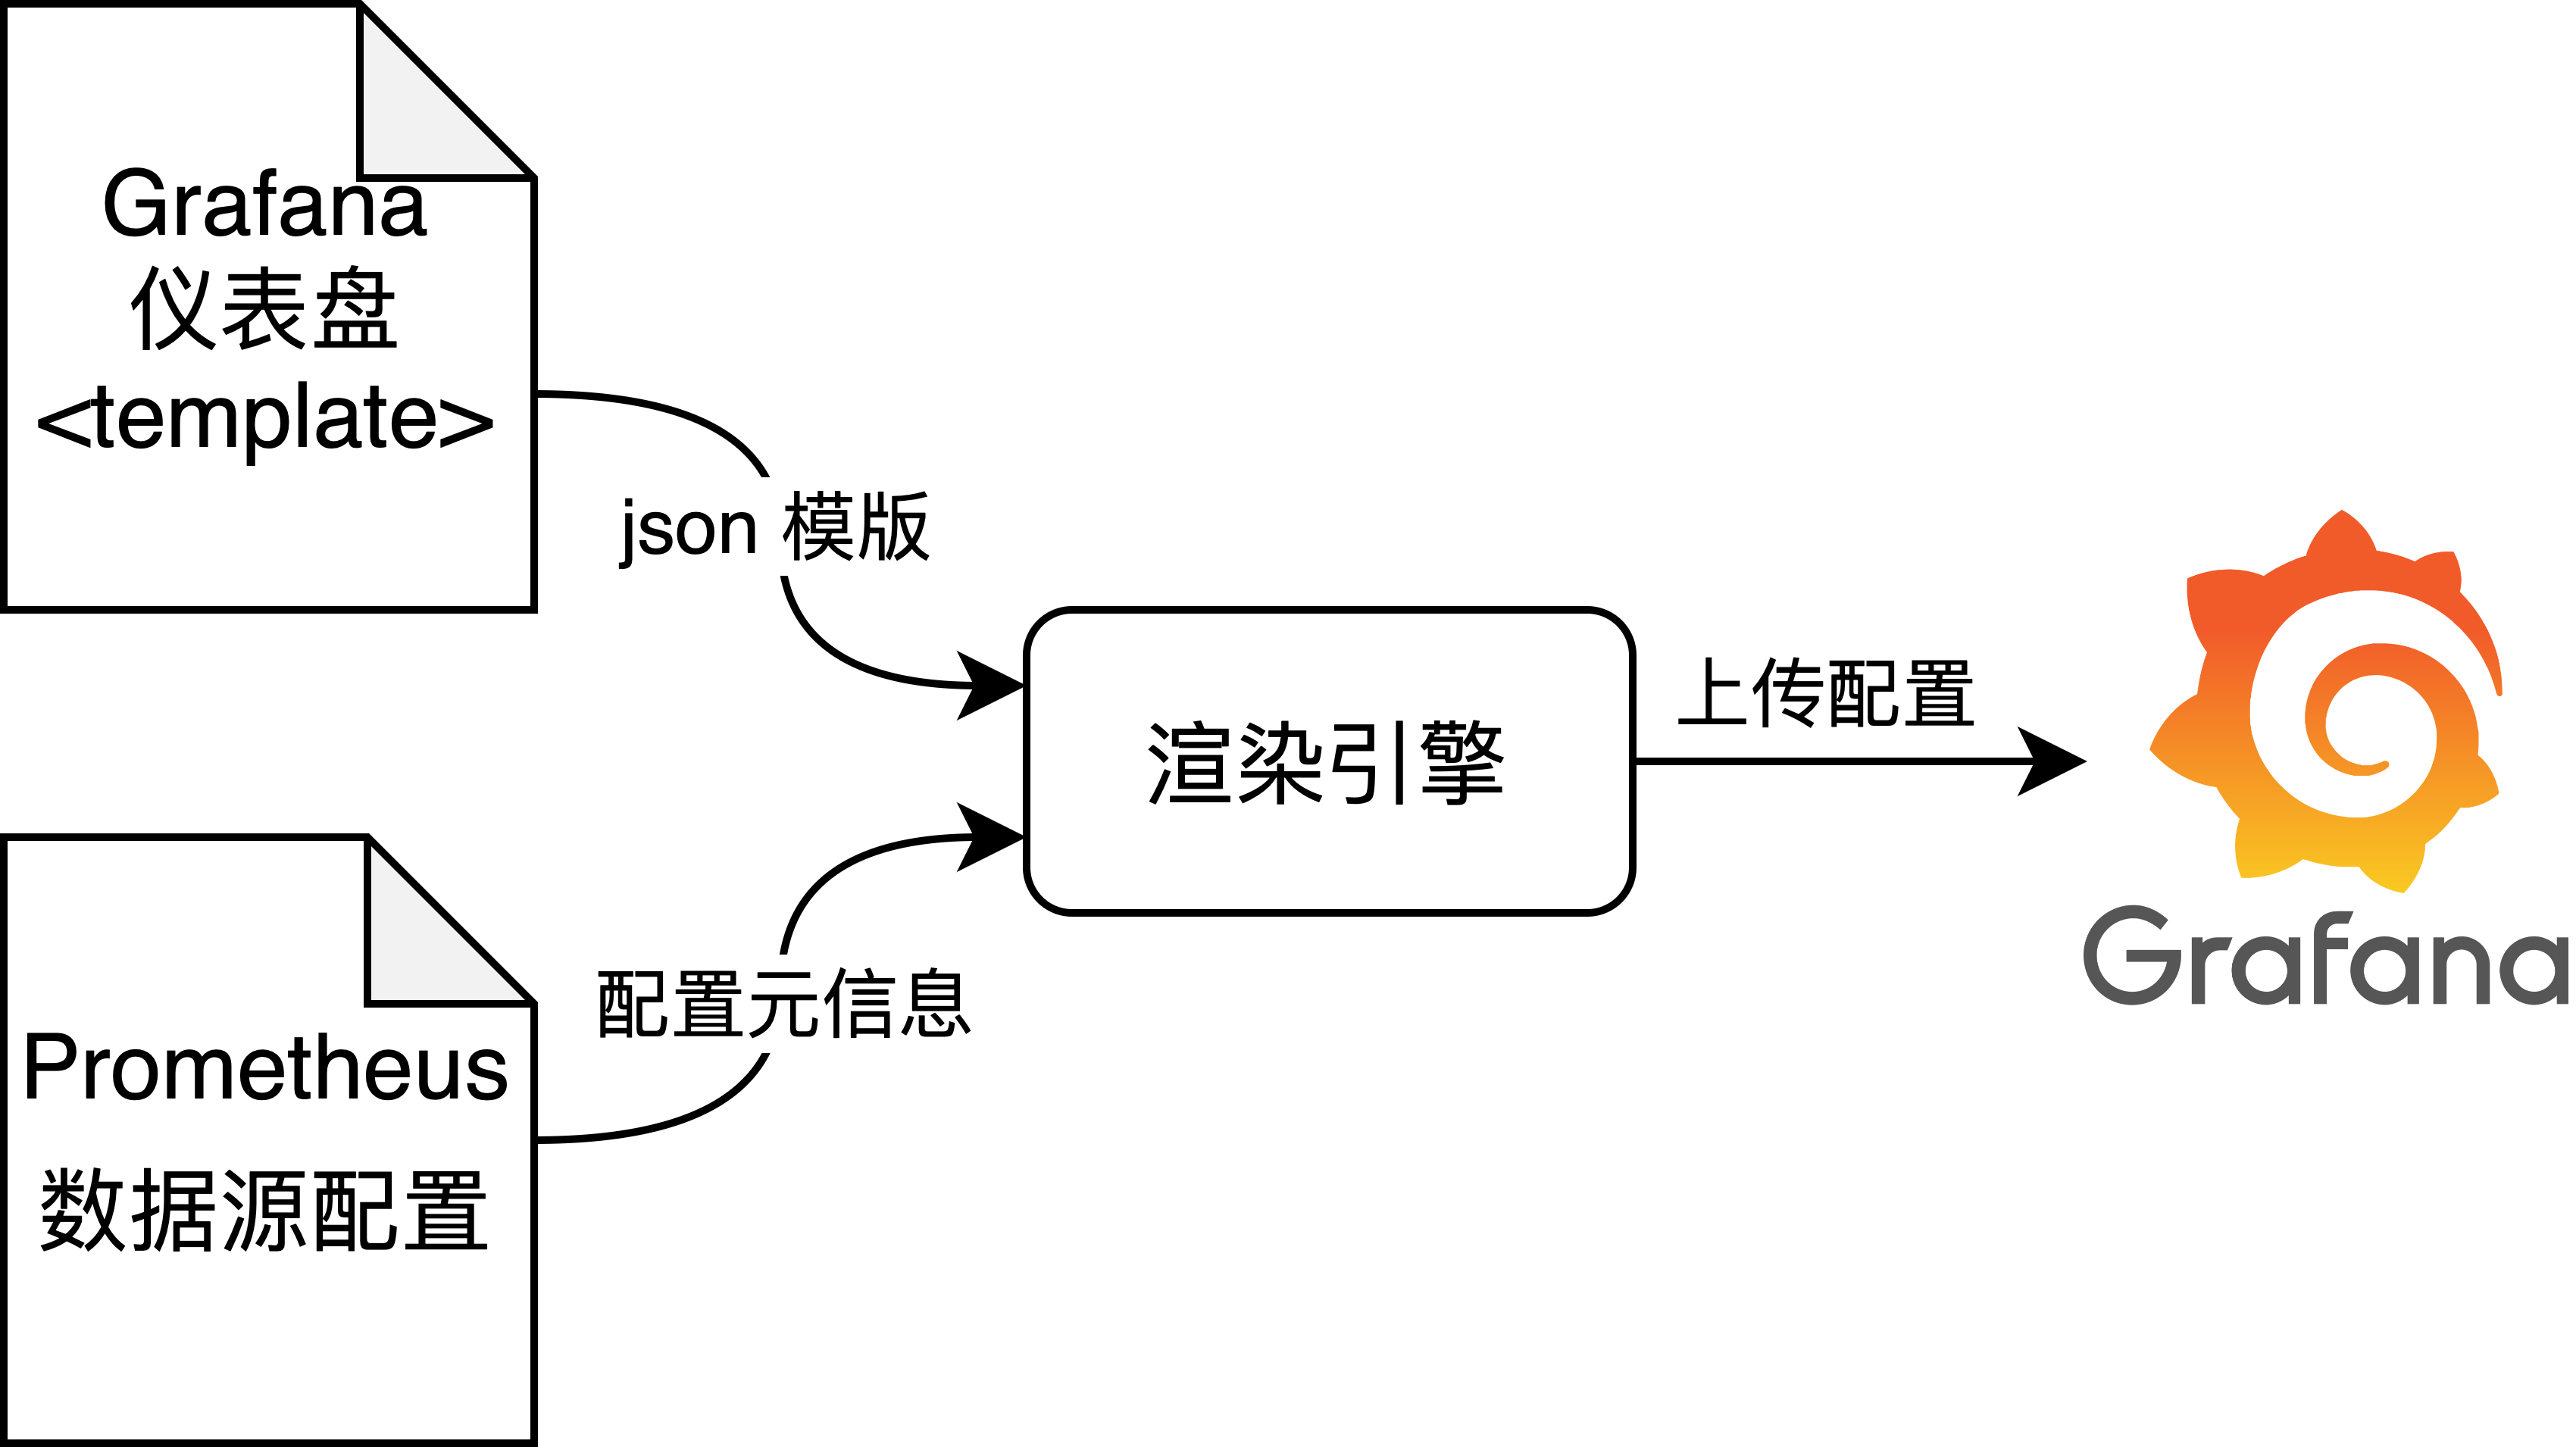
\includegraphics[width=0.65\linewidth]{pics/4-12grafana.png}
  \caption{监控数据可视化架构}
  \label{fig:4-12grafana}
\end{figure}

边缘节点的监控数据通过每一层的边缘节点逐步汇总,最终传输至云端。这一过程不仅有效减少了云边之间的冗余数据传输开销,还为边缘侧的实时调度提供了必要的数据支持。在云端,本文集成了Prometheus和Grafana数据可视化平台。如图\ref{fig:4-12grafana}所示,收集到的数据首先存储在Prometheus中。Prometheus作为一个强大的时间序列数据库,能够高效地存储和查询大量的监控数据。然后,通过预定义的Grafana仪表盘模板文件,填充相应的Prometheus数据源配置信息。这些模板文件包含了各种图表、面板和告警规则,可以根据实际需求进行灵活配置。最后,这些配置被上传到Grafana仪表盘,利用丰富的可视化组件提供直观的监控视图。这种可视化的方式使得相关人员能够快速掌握系统的运行状态,及时发现并处理潜在的问题,从而提高系统的整体可靠性和性能。

\section{本章小结}

本章介绍了云边协同AI推理调度系统的设计与实现。首先,详细阐述了KubeEdge及相关技术,包括其架构设计、设备管理机制以及EdgeMesh的服务通信机制。接着,对系统的整体架构进行了说明,明确了各组件在系统中的功能定位及其相互协作关系。最后,深入探讨了系统中各个关键组件的设计与实现细节,描述了这些组件如何为前文提出的调度算法提供系统支撑,从而确保云边协同环境下模型推理任务的高效调度与执行。

